% E03. Regimen hidroclimatico.
% Va en el dossier en lugar de la seccion E03 de la plantilla:
%   % E03. Regimen hidroclimatico.
% Va en el dossier en lugar de la seccion E03 de la plantilla:
%   % E03. Regimen hidroclimatico.
% Va en el dossier en lugar de la seccion E03 de la plantilla:
%   % E03. Regimen hidroclimatico.
% Va en el dossier en lugar de la seccion E03 de la plantilla:
%   \input{evidencias/E03_regimen_hidroclimatico}
% Cifras: 03_outputs/tables/05_climatologia_mensual.csv, 05_regimen_mensual_P_PET_Q.csv,
% 05_resumen_regimen_E03.csv, 05_indice_aridez.csv, 05_mapas_rango_en_cuenca.csv,
% 05_koppen_cuenca.csv y 05_relaciones_anuales_E04.csv, generadas por run_all.R.
% Periodo 1987-2019, poligono de Alexis, caudal rellenado.

\section{E03. Régimen hidroclimático}
\label{ev:E03}

\campo{1. Pregunta o afirmación que se evalúa}{¿Qué estacionalidad y qué
procesos dominan el régimen de la cuenca?}

\campo{2. Evidencia principal}{El climograma (Figura~\ref{fig:E03climograma})
y el régimen mensual de P, PET y Q (Figura~\ref{fig:E03regimen}), con sus
valores en la Tabla~\ref{tab:E03mensual}. La Tabla~\ref{tab:E03indices}
resume los índices anuales, la Figura~\ref{fig:E03mapas} muestra la P y la
Tmed anuales en la grilla de CR2MET y la Figura~\ref{fig:E03koppen}, la
clasificación de Köppen-Geiger. Todo para 1987--2019: 33 años, 396 meses por
variable.}

\begin{figure}[ht]
\centering
\IfFileExists{../03_outputs/figures/05_climograma.png}{%
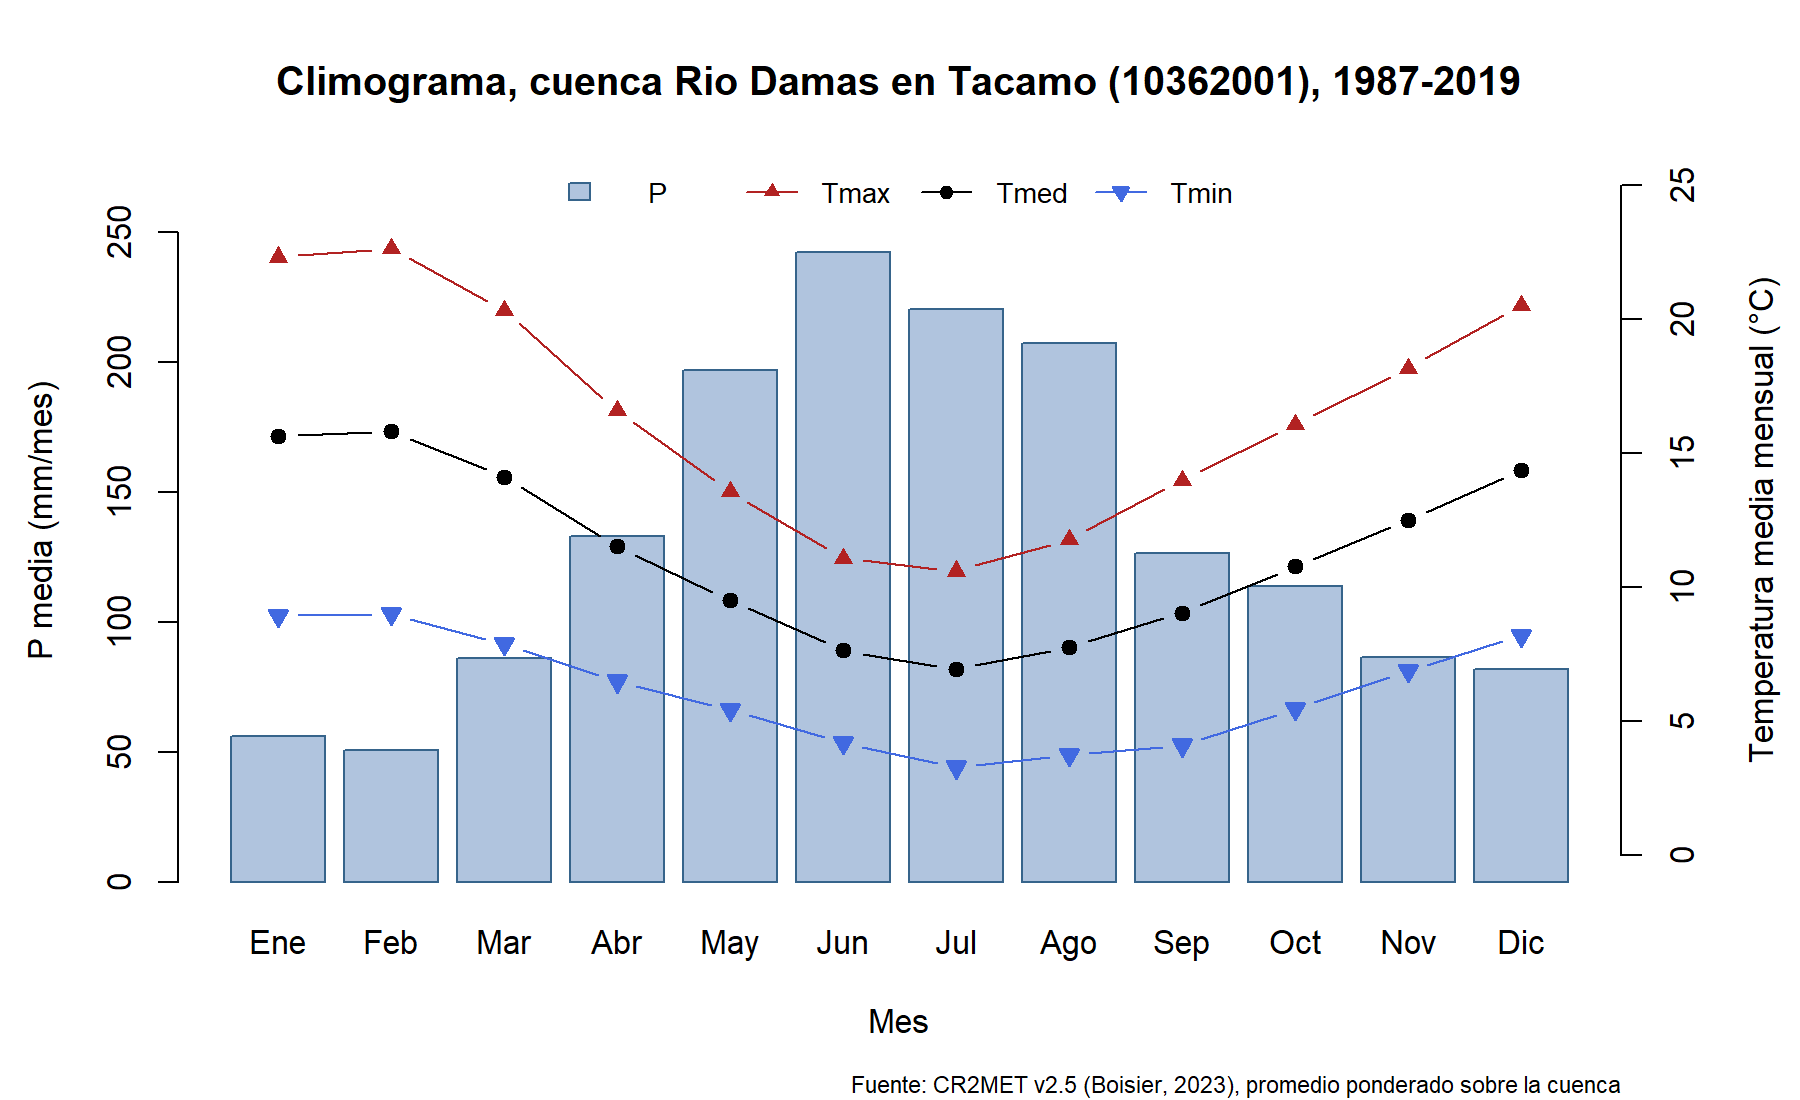
\includegraphics[width=0.85\textwidth]{../03_outputs/figures/05_climograma.png}}{%
\fbox{Falta 03\_outputs/figures/05\_climograma.png}}
\caption{Climograma de la cuenca, 1987--2019: P media mensual (barras,
mm\,mes$^{-1}$) y Tmax, Tmed y Tmin medias mensuales (líneas, °C), de CR2MET
v2.5 \citep{Boisier2023} promediado sobre la cuenca.}
\label{fig:E03climograma}
\end{figure}

\begin{figure}[ht]
\centering
\IfFileExists{../03_outputs/figures/05_regimen_P_PET_Q.png}{%
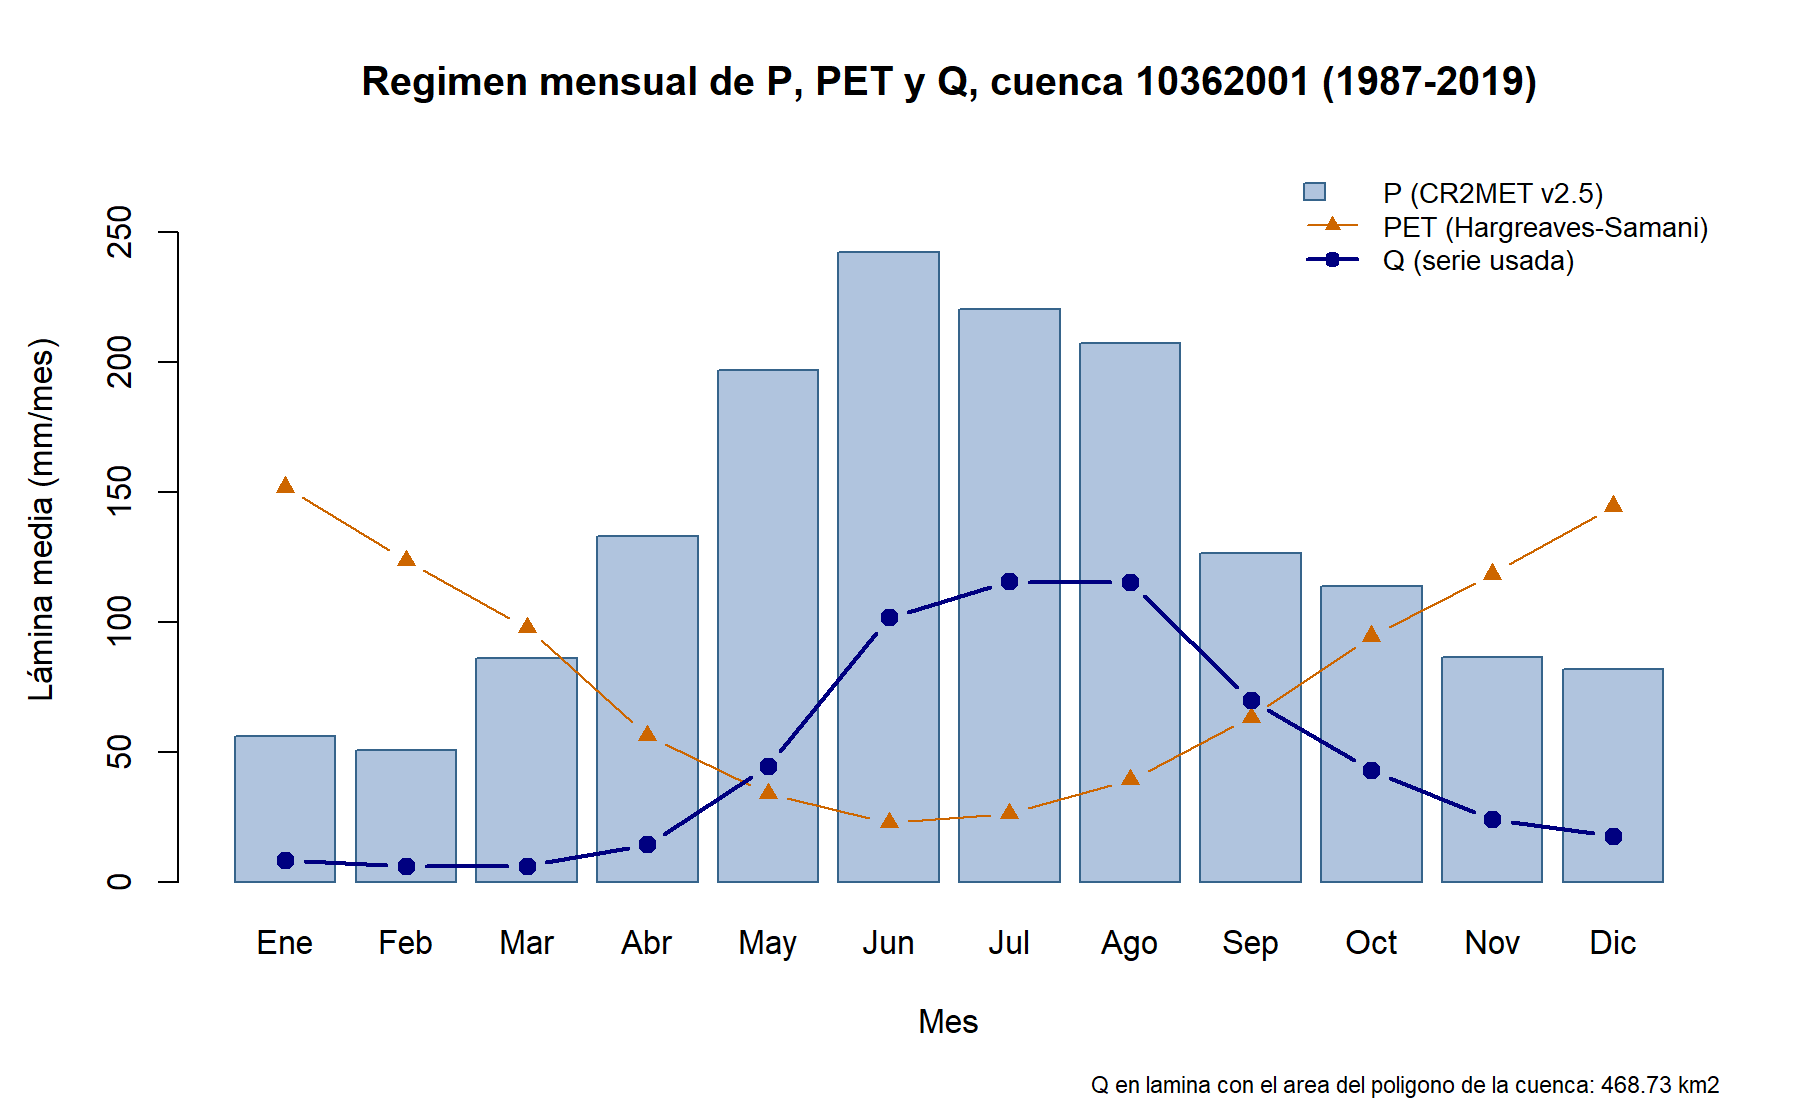
\includegraphics[width=0.85\textwidth]{../03_outputs/figures/05_regimen_P_PET_Q.png}}{%
\fbox{Falta 03\_outputs/figures/05\_regimen\_P\_PET\_Q.png}}
\caption{Régimen mensual de P, PET y Q en lámina (mm\,mes$^{-1}$),
1987--2019. Q es el caudal DGA rellenado por el integrante 2 (E02), pasado a
lámina con el área de la cuenca de E01 (468.73 km$^2$) según la
ecuación~(\ref{eq:E03lamina}).}
\label{fig:E03regimen}
\end{figure}

\begin{table}[ht]
\centering
\caption{Valores medios mensuales, 1987--2019 (33 años). P, PET y Q en
mm\,mes$^{-1}$; Q/P adimensional; temperaturas en °C. La fila del año suma
los valores sin redondear (P, PET y Q en mm\,año$^{-1}$) y da la media anual
de las temperaturas.}
\label{tab:E03mensual}
\begin{tabular}{|l|r|r|r|r|r|r|r|}
\hline
Mes & P & PET & Q & Q/P & Tmax & Tmed & Tmin \\
\hline
Ene & 56.3 & 152.0 & 8.3 & 0.15 & 22.31 & 15.61 & 8.92 \\
\hline
Feb & 50.6 & 123.8 & 6.0 & 0.12 & 22.63 & 15.81 & 9.00 \\
\hline
Mar & 86.2 & 98.0 & 6.2 & 0.07 & 20.32 & 14.10 & 7.87 \\
\hline
Abr & 133.1 & 56.4 & 14.4 & 0.11 & 16.57 & 11.52 & 6.48 \\
\hline
May & 196.8 & 34.0 & 44.4 & 0.23 & 13.55 & 9.49 & 5.43 \\
\hline
Jun & 242.3 & 22.9 & 101.7 & 0.42 & 11.07 & 7.63 & 4.18 \\
\hline
Jul & 220.5 & 26.2 & 115.6 & 0.52 & 10.60 & 6.93 & 3.27 \\
\hline
Ago & 207.3 & 39.3 & 115.4 & 0.56 & 11.77 & 7.76 & 3.75 \\
\hline
Sep & 126.5 & 63.3 & 69.8 & 0.55 & 13.98 & 9.04 & 4.10 \\
\hline
Oct & 113.8 & 94.6 & 42.8 & 0.38 & 16.07 & 10.76 & 5.45 \\
\hline
Nov & 86.5 & 118.4 & 24.1 & 0.28 & 18.16 & 12.51 & 6.87 \\
\hline
Dic & 81.9 & 144.6 & 17.5 & 0.21 & 20.49 & 14.34 & 8.18 \\
\hline
Año & 1601.6 & 973.4 & 566.1 & 0.35 & 16.43 & 11.27 & 6.11 \\
\hline
\end{tabular}
\end{table}

\begin{table}[ht]
\centering
\caption{Índices del período 1987--2019. Las razones son adimensionales.}
\label{tab:E03indices}
\begin{tabular}{|p{0.5\linewidth}|p{0.35\linewidth}|}
\hline
Indicador & Valor \\
\hline
P media anual & 1601.6 mm\,año$^{-1}$ \\
\hline
PET media anual \citep{Hargreaves1985} & 973.4 mm\,año$^{-1}$ \\
\hline
Q medio anual & 566.1 mm\,año$^{-1}$ (8.41 m$^3$\,s$^{-1}$) \\
\hline
Índice de aridez PET/P, ecuación~(\ref{eq:E03aridez}) & 0.608 \\
\hline
Coeficiente de escorrentía Q/P, ecuación~(\ref{eq:E03aridez}) & 0.353 \\
\hline
ET real por balance sobre P, (P $-$ Q)/P & 0.647 \\
\hline
P de mayo a agosto & 54.1 \% del año \\
\hline
Q de mayo a agosto & 66.6 \% del año \\
\hline
Meses con PET mayor que P & enero, febrero, marzo, noviembre y diciembre \\
\hline
P media anual en las celdas de 0.05° que tocan la cuenca & 1291.3 a 2034.4 mm\,año$^{-1}$ \\
\hline
Tmed anual en las celdas de 0.05° que tocan la cuenca & 10.9 a 11.6 °C \\
\hline
Köppen-Geiger 1991--2020 \citep{Beck2023}, \% del área & Cfb 92.6; Csb 7.4 \\
\hline
\end{tabular}
\end{table}

\begin{figure}[ht]
\centering
\IfFileExists{../03_outputs/figures/05_mapas_P_T_media_anual.png}{%
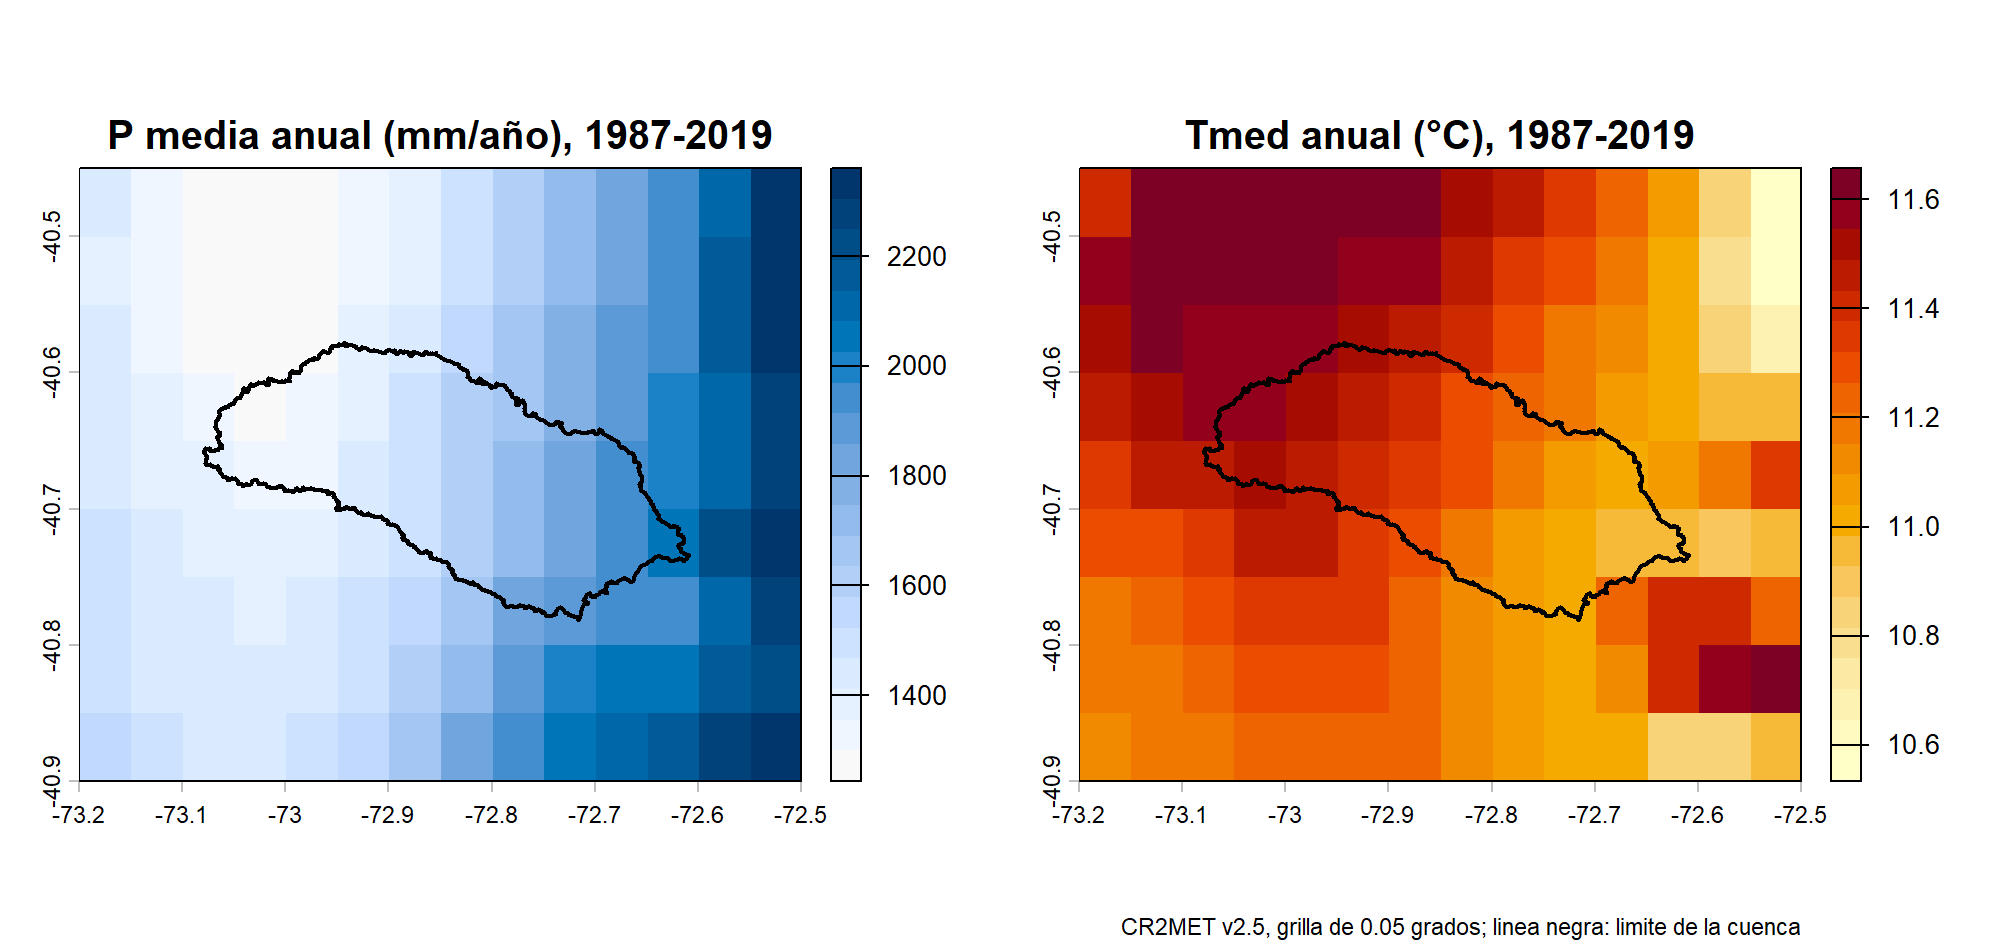
\includegraphics[width=0.95\textwidth]{../03_outputs/figures/05_mapas_P_T_media_anual.png}}{%
\fbox{Falta 03\_outputs/figures/05\_mapas\_P\_T\_media\_anual.png}}
\caption{P media anual (mm\,año$^{-1}$) y Tmed anual (°C) de CR2MET v2.5,
1987--2019, en la grilla de 0.05° (coordenadas geográficas WGS84,
EPSG:4326). La línea negra es el límite de la cuenca.}
\label{fig:E03mapas}
\end{figure}

\begin{figure}[ht]
\centering
\IfFileExists{../03_outputs/figures/05_mapa_koppen.png}{%
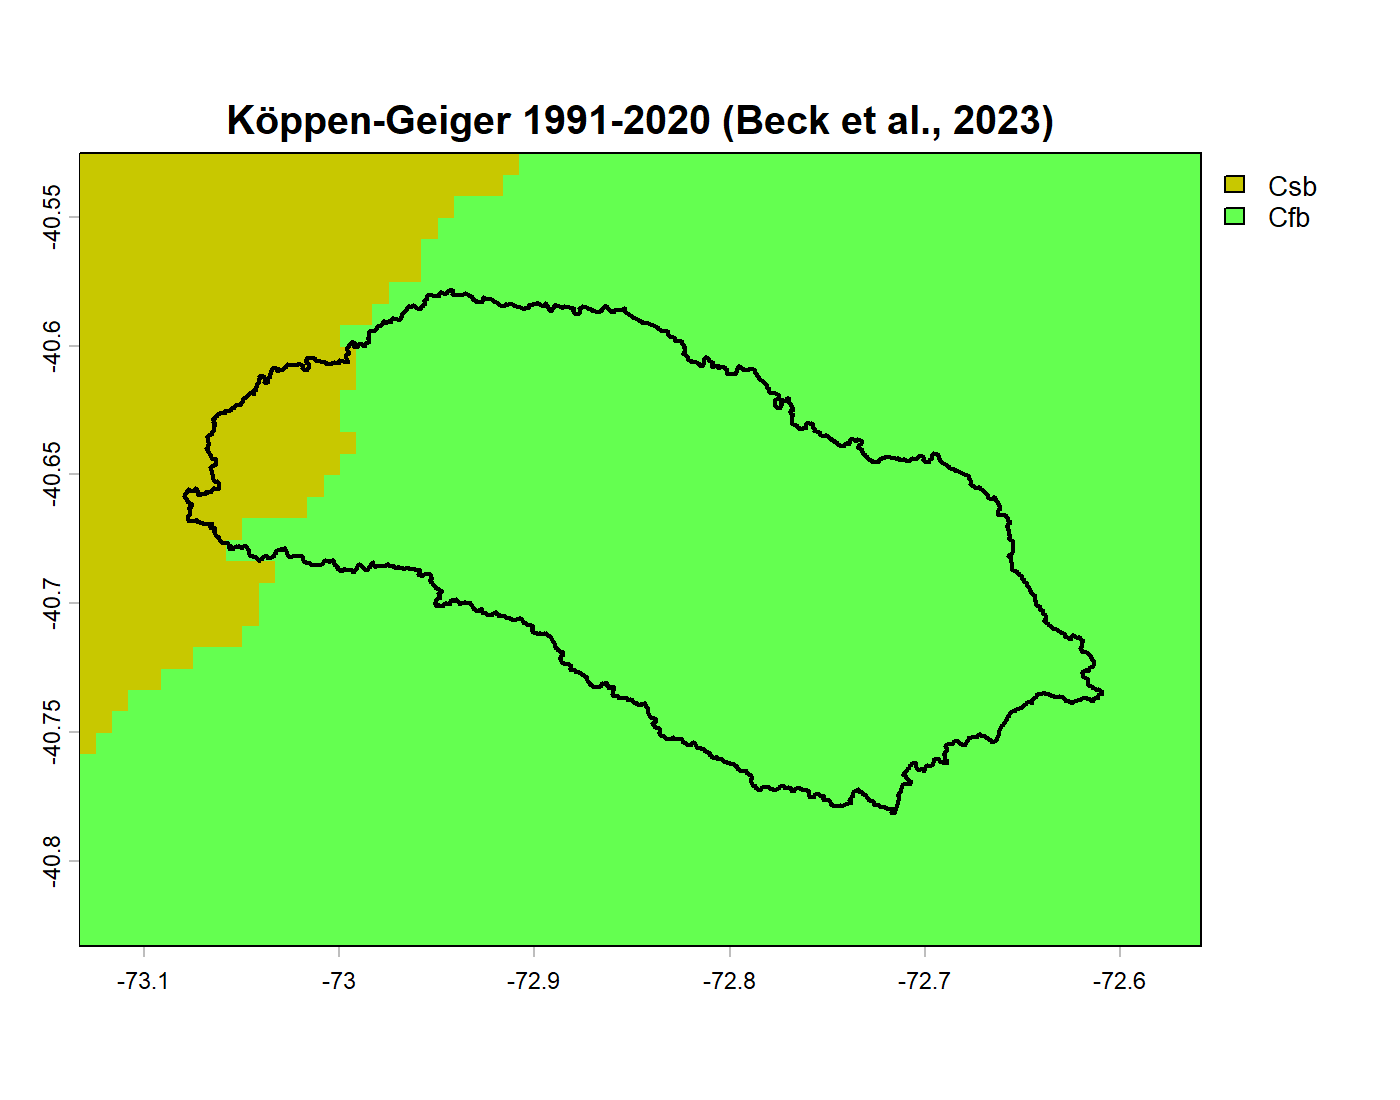
\includegraphics[width=0.7\textwidth]{../03_outputs/figures/05_mapa_koppen.png}}{%
\fbox{Falta 03\_outputs/figures/05\_mapa\_koppen.png}}
\caption{Clasificación de Köppen-Geiger 1991--2020 de \citet{Beck2023}, en
la grilla de 1 km (coordenadas geográficas WGS84). Cfb: templado, sin
estación seca y con verano templado. Csb: templado, con verano seco y
templado. La línea negra es el límite de la cuenca.}
\label{fig:E03koppen}
\end{figure}

\campo{3. Fuente y trazabilidad}{P, Tmax y Tmin vienen de CR2MET v2.5
\citep{Boisier2023} (grilla de 0.05°, WGS84) y la PET de
\citet{Hargreaves1985}, todo promediado sobre el polígono de la cuenca de E01
(ver E02). El caudal es la serie DGA rellenada por el integrante 2.
\texttt{02\_\allowbreak{}Rscripts/\allowbreak{}05\_\allowbreak{}regimen\_\allowbreak{}hidroclimatico.R} agrega a escala mensual
(P, PET y Q se suman, las temperaturas se promedian), promedia cada mes del
año en 1987--2019, recorta el mapa de Köppen-Geiger y escribe las cifras en
\texttt{03\_\allowbreak{}outputs/\allowbreak{}tables/\allowbreak{}} (\texttt{05\_\allowbreak{}climatologia\_\allowbreak{}mensual.csv},
\texttt{05\_\allowbreak{}regimen\_\allowbreak{}mensual\_\allowbreak{}P\_\allowbreak{}PET\_\allowbreak{}Q.csv},
\texttt{05\_\allowbreak{}resumen\_\allowbreak{}regimen\_\allowbreak{}E03.csv}, \texttt{05\_\allowbreak{}indice\_\allowbreak{}aridez.csv},
\texttt{05\_\allowbreak{}mapas\_\allowbreak{}rango\_\allowbreak{}en\_\allowbreak{}cuenca.csv} y \texttt{05\_\allowbreak{}koppen\_\allowbreak{}cuenca.csv}) y
las figuras en \texttt{03\_\allowbreak{}outputs/\allowbreak{}figures/\allowbreak{}} (\texttt{05\_\allowbreak{}climograma.png},
\texttt{05\_\allowbreak{}regimen\_\allowbreak{}P\_\allowbreak{}PET\_\allowbreak{}Q.png}, \texttt{05\_\allowbreak{}mapas\_\allowbreak{}P\_\allowbreak{}T\_\allowbreak{}media\_\allowbreak{}anual.png}
y \texttt{05\_\allowbreak{}mapa\_\allowbreak{}koppen.png}). Los mapas de P y T se rehacen solo donde
están las grillas de CR2MET; el de Köppen se rehace desde el recorte que
queda en \texttt{01\_\allowbreak{}data/\allowbreak{}processed/\allowbreak{}}. Las fuentes están en
\texttt{04\_\allowbreak{}metadata/\allowbreak{}data\_\allowbreak{}sources.csv}, el período en
\texttt{06\_\allowbreak{}config/\allowbreak{}parametros.csv}, y todo se regenera con
\texttt{run\_\allowbreak{}all.R}.}

\campo{4. Interpretación hidrológica}{El régimen es pluvial. La P se concentra
entre mayo y agosto (54.1 \% del año, máximo en junio) y el caudal la sigue
con uno o dos meses de retraso: el máximo es en julio y agosto, y entre mayo y
agosto pasa el 66.6 \% del caudal anual. No hay un segundo máximo en
primavera, que sería la señal de un aporte nival, y la cuenca es baja
(cotas bajo 350 m, E01). En septiembre el cociente Q/P sigue tan alto como en
agosto (0.55 y 0.56), lo que sugiere un almacenamiento que se vacía después
del invierno, aunque con esta evidencia no se puede decir dónde está (suelo,
acuífero o lagos).

En verano el clima pasa a estar limitado por agua: de noviembre a marzo la
PET supera a la P, el caudal cae a 6 mm\,mes$^{-1}$ en febrero y marzo y la
razón entre el mes de más caudal y el de menos es 19. A escala anual la
cuenca está limitada por energía, con PET/P = 0.608, menor que 1. La
clasificación de Köppen-Geiger es coherente con ese cuadro: el 92.6 \% del
área es Cfb (templado, sin estación seca) y solo el borde oeste, cerca de
Osorno, es Csb (con verano seco). La P de CR2MET aumenta de oeste a este
dentro de la cuenca, mientras la Tmed casi no varía.}

\campo{5. Consistencia física}{El índice de aridez usado es el cociente
PET/P del enfoque de Budyko \citep{Sposito2017}, el mismo de E06, y el
caudal en lámina sale de dividir el volumen por el área:
\begin{equation}
\phi = \frac{\mathrm{PET}}{P}, \qquad
c_Q = \frac{Q}{P}
\label{eq:E03aridez}
\end{equation}
\begin{equation}
Q_{\mathrm{mm/d}} = \frac{86{.}4\, Q_{\mathrm{m^3/s}}}{A_{\mathrm{km^2}}}
\label{eq:E03lamina}
\end{equation}
P, PET y Q se suman en el mes y las temperaturas se promedian; la fila anual
de la Tabla~\ref{tab:E03mensual} cierra con los totales. La PET es máxima en
enero y mínima en junio, como la radiación extraterrestre que usa la
ecuación de Hargreaves, y va un mes antes que la Tmed (máxima en febrero,
mínima en julio). Tmin queda siempre bajo Tmed y Tmed bajo Tmax. Hay una
inconsistencia que se arrastra a E06: la ET real que deja el balance,
(P $-$ Q)/P = 0.647, es mayor que PET/P = 0.608, así que el punto de la
cuenca queda sobre el límite de energía de Budyko (ver E04 y E06).}

\campo{6. Limitaciones e incertidumbre}{La P y la T son de un producto
grillado de 0.05° (unos 5 km) y no de estaciones dentro de la cuenca, así que
el gradiente de P hacia el este depende de cómo CR2MET reparte la lluvia; el
rango de la Tabla~\ref{tab:E03indices} incluye celdas que solo tocan el
borde de la cuenca. El caudal de 11 de los 33 años incluye días rellenados
(E02). Entre ellos hay 19 días de verano de 2014--2015 en 0 m$^3$\,s$^{-1}$,
que son un artefacto de la regresión y no un caudal observado. El rol del
almacenamiento en la recesión de primavera es una inferencia del desfase
entre P y Q, no una observación. El mapa de Köppen-Geiger es de 1991--2020 y
no de 1987--2019.}

\campo{7. Conclusión asociada}{En 1987--2019 la cuenca del Río Damas en
Tacamo tiene un régimen pluvial: la lluvia de otoño e invierno (máximo en
junio) produce el máximo de caudal en julio y agosto, y en verano la PET
supera a la P y el caudal baja a su mínimo. A escala anual la cuenca está
limitada por energía (PET/P = 0.608) y su clima es templado sin estación
seca (Cfb en el 92.6 \% del área).}

% Cifras: 03_outputs/tables/05_climatologia_mensual.csv, 05_regimen_mensual_P_PET_Q.csv,
% 05_resumen_regimen_E03.csv, 05_indice_aridez.csv, 05_mapas_rango_en_cuenca.csv,
% 05_koppen_cuenca.csv y 05_relaciones_anuales_E04.csv, generadas por run_all.R.
% Periodo 1987-2019, poligono de Alexis, caudal rellenado.

\section{E03. Régimen hidroclimático}
\label{ev:E03}

\campo{1. Pregunta o afirmación que se evalúa}{¿Qué estacionalidad y qué
procesos dominan el régimen de la cuenca?}

\campo{2. Evidencia principal}{El climograma (Figura~\ref{fig:E03climograma})
y el régimen mensual de P, PET y Q (Figura~\ref{fig:E03regimen}), con sus
valores en la Tabla~\ref{tab:E03mensual}. La Tabla~\ref{tab:E03indices}
resume los índices anuales, la Figura~\ref{fig:E03mapas} muestra la P y la
Tmed anuales en la grilla de CR2MET y la Figura~\ref{fig:E03koppen}, la
clasificación de Köppen-Geiger. Todo para 1987--2019: 33 años, 396 meses por
variable.}

\begin{figure}[ht]
\centering
\IfFileExists{../03_outputs/figures/05_climograma.png}{%
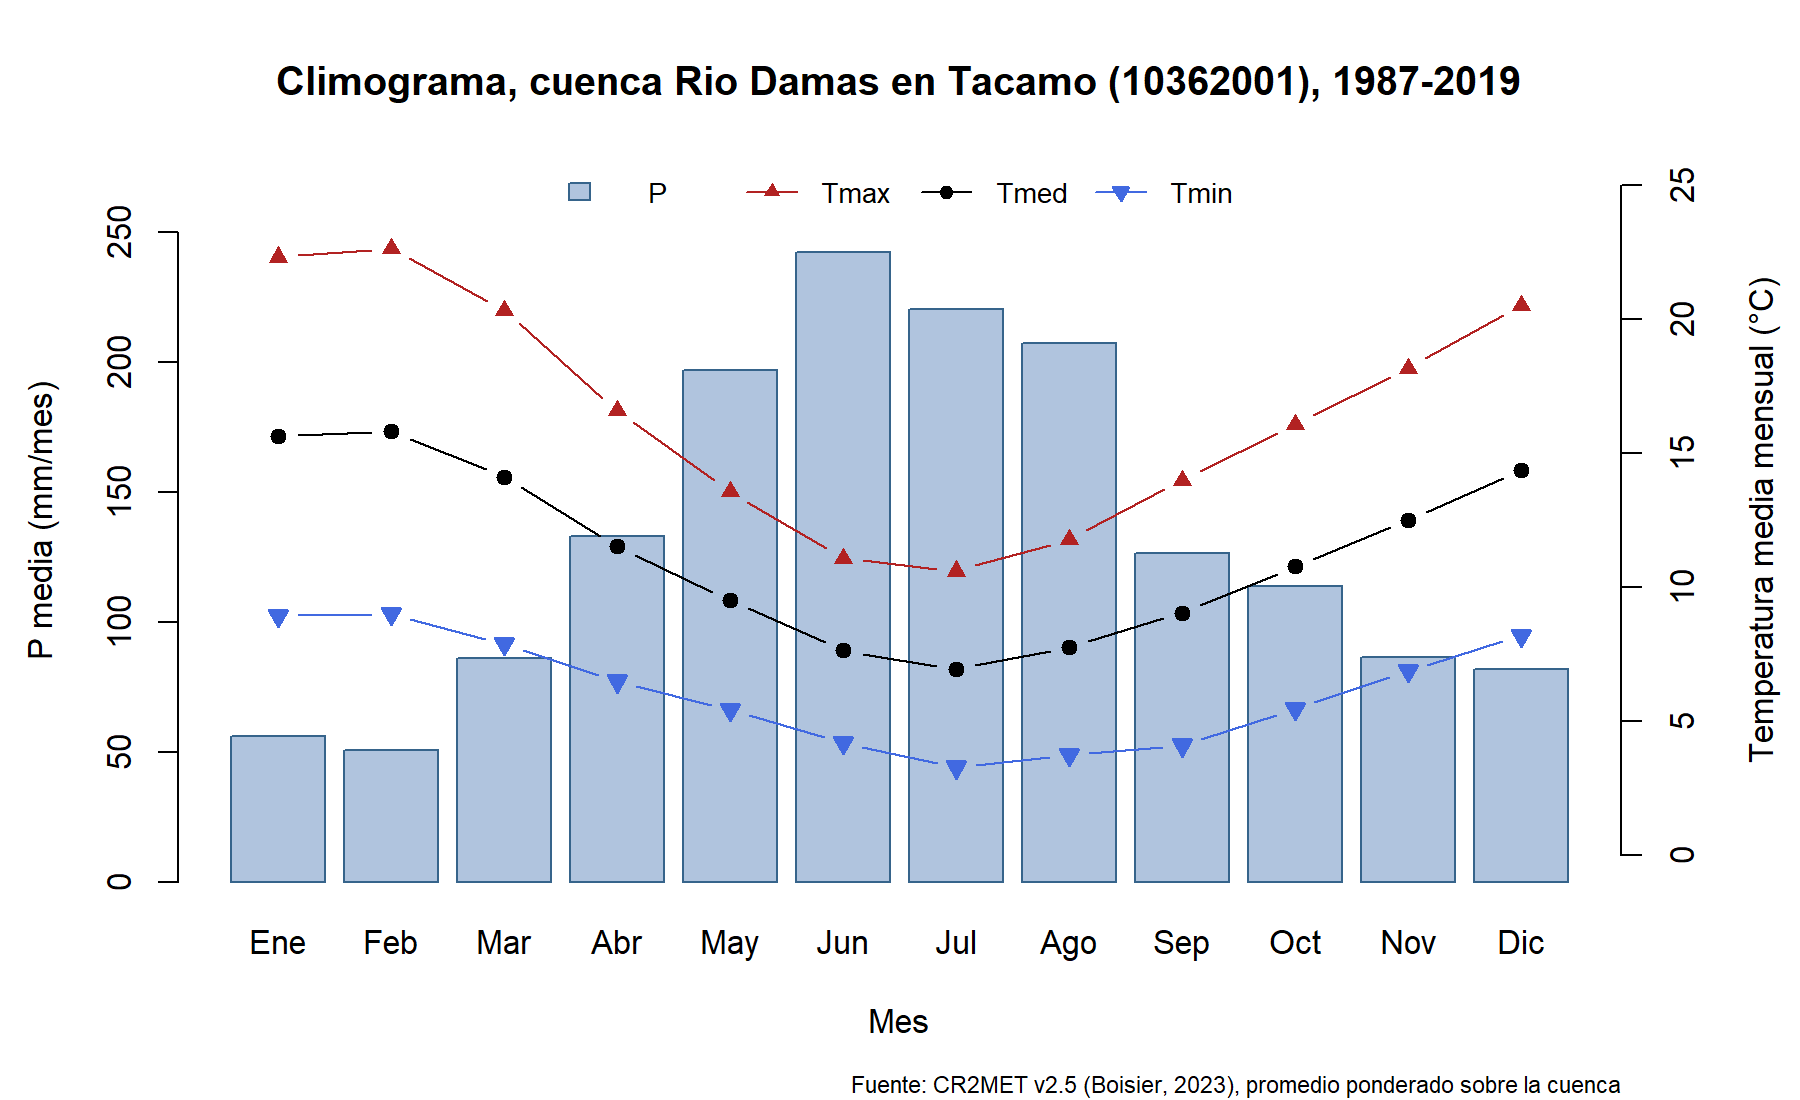
\includegraphics[width=0.85\textwidth]{../03_outputs/figures/05_climograma.png}}{%
\fbox{Falta 03\_outputs/figures/05\_climograma.png}}
\caption{Climograma de la cuenca, 1987--2019: P media mensual (barras,
mm\,mes$^{-1}$) y Tmax, Tmed y Tmin medias mensuales (líneas, °C), de CR2MET
v2.5 \citep{Boisier2023} promediado sobre la cuenca.}
\label{fig:E03climograma}
\end{figure}

\begin{figure}[ht]
\centering
\IfFileExists{../03_outputs/figures/05_regimen_P_PET_Q.png}{%
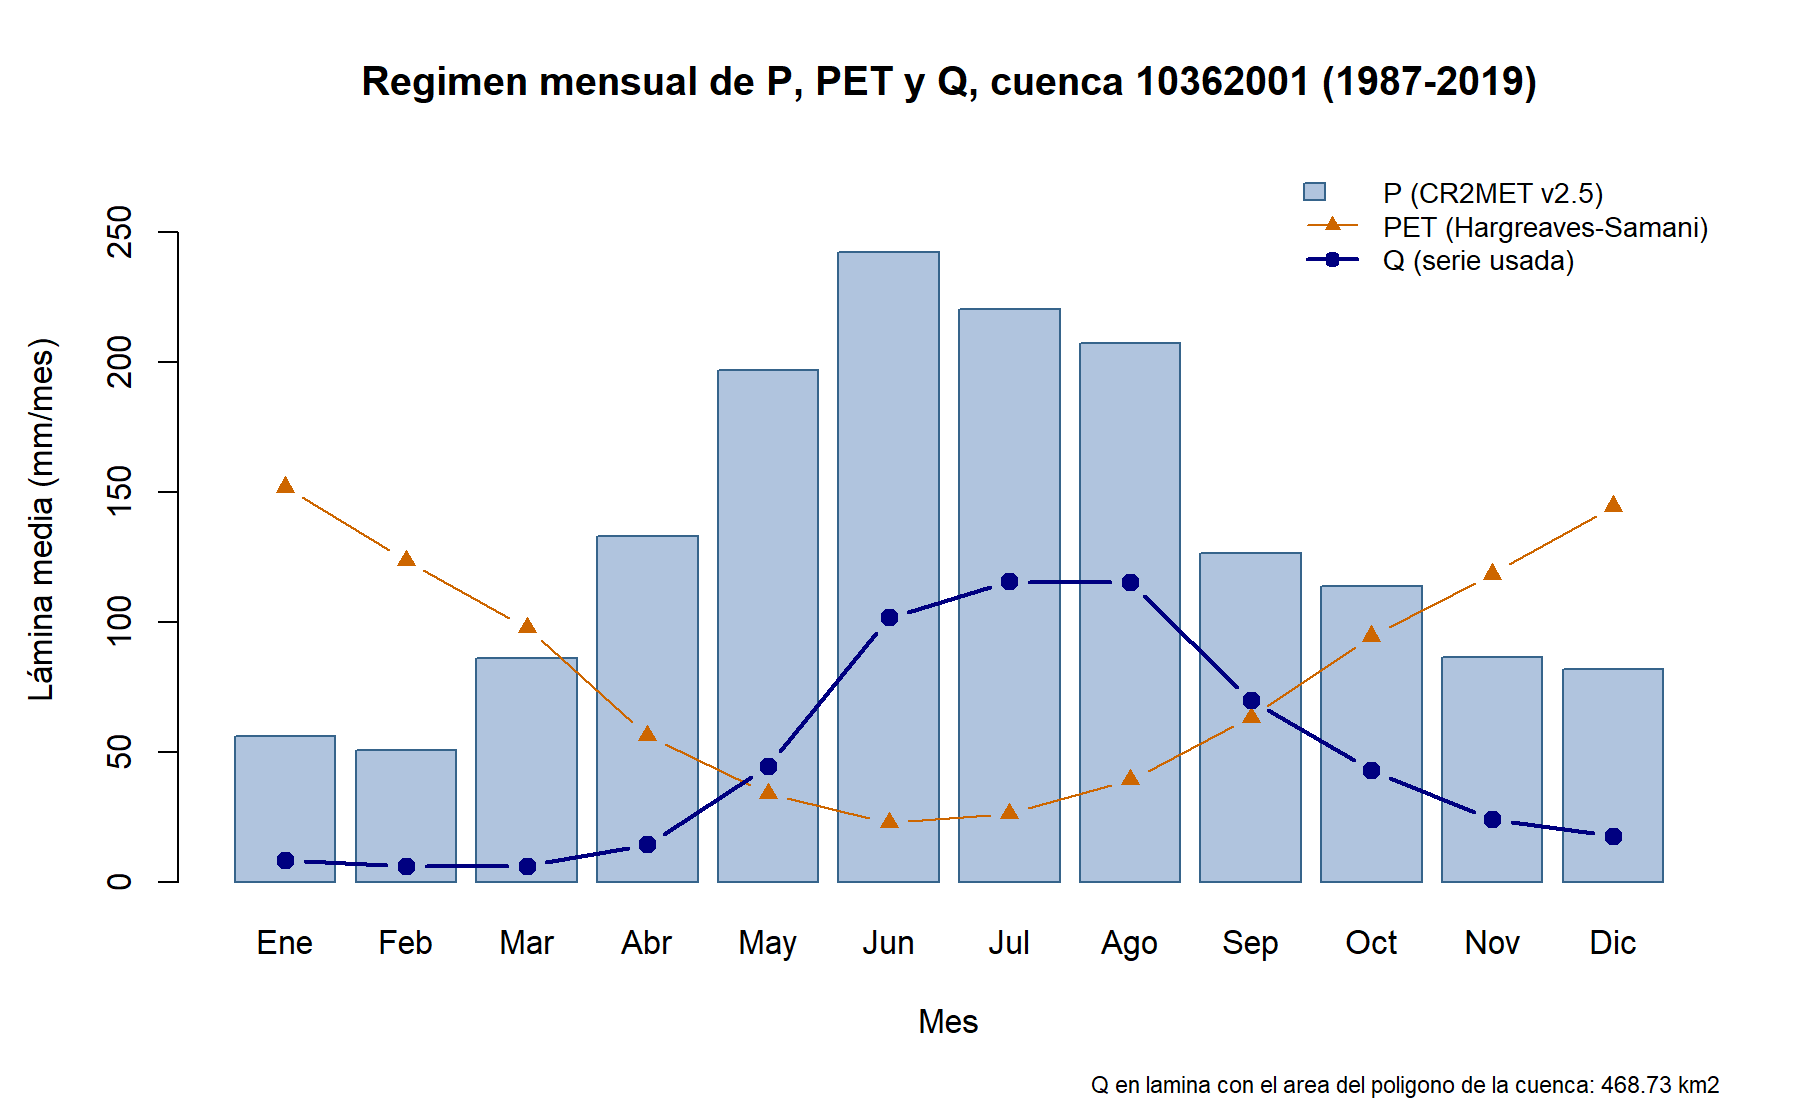
\includegraphics[width=0.85\textwidth]{../03_outputs/figures/05_regimen_P_PET_Q.png}}{%
\fbox{Falta 03\_outputs/figures/05\_regimen\_P\_PET\_Q.png}}
\caption{Régimen mensual de P, PET y Q en lámina (mm\,mes$^{-1}$),
1987--2019. Q es el caudal DGA rellenado por el integrante 2 (E02), pasado a
lámina con el área de la cuenca de E01 (468.73 km$^2$) según la
ecuación~(\ref{eq:E03lamina}).}
\label{fig:E03regimen}
\end{figure}

\begin{table}[ht]
\centering
\caption{Valores medios mensuales, 1987--2019 (33 años). P, PET y Q en
mm\,mes$^{-1}$; Q/P adimensional; temperaturas en °C. La fila del año suma
los valores sin redondear (P, PET y Q en mm\,año$^{-1}$) y da la media anual
de las temperaturas.}
\label{tab:E03mensual}
\begin{tabular}{|l|r|r|r|r|r|r|r|}
\hline
Mes & P & PET & Q & Q/P & Tmax & Tmed & Tmin \\
\hline
Ene & 56.3 & 152.0 & 8.3 & 0.15 & 22.31 & 15.61 & 8.92 \\
\hline
Feb & 50.6 & 123.8 & 6.0 & 0.12 & 22.63 & 15.81 & 9.00 \\
\hline
Mar & 86.2 & 98.0 & 6.2 & 0.07 & 20.32 & 14.10 & 7.87 \\
\hline
Abr & 133.1 & 56.4 & 14.4 & 0.11 & 16.57 & 11.52 & 6.48 \\
\hline
May & 196.8 & 34.0 & 44.4 & 0.23 & 13.55 & 9.49 & 5.43 \\
\hline
Jun & 242.3 & 22.9 & 101.7 & 0.42 & 11.07 & 7.63 & 4.18 \\
\hline
Jul & 220.5 & 26.2 & 115.6 & 0.52 & 10.60 & 6.93 & 3.27 \\
\hline
Ago & 207.3 & 39.3 & 115.4 & 0.56 & 11.77 & 7.76 & 3.75 \\
\hline
Sep & 126.5 & 63.3 & 69.8 & 0.55 & 13.98 & 9.04 & 4.10 \\
\hline
Oct & 113.8 & 94.6 & 42.8 & 0.38 & 16.07 & 10.76 & 5.45 \\
\hline
Nov & 86.5 & 118.4 & 24.1 & 0.28 & 18.16 & 12.51 & 6.87 \\
\hline
Dic & 81.9 & 144.6 & 17.5 & 0.21 & 20.49 & 14.34 & 8.18 \\
\hline
Año & 1601.6 & 973.4 & 566.1 & 0.35 & 16.43 & 11.27 & 6.11 \\
\hline
\end{tabular}
\end{table}

\begin{table}[ht]
\centering
\caption{Índices del período 1987--2019. Las razones son adimensionales.}
\label{tab:E03indices}
\begin{tabular}{|p{0.5\linewidth}|p{0.35\linewidth}|}
\hline
Indicador & Valor \\
\hline
P media anual & 1601.6 mm\,año$^{-1}$ \\
\hline
PET media anual \citep{Hargreaves1985} & 973.4 mm\,año$^{-1}$ \\
\hline
Q medio anual & 566.1 mm\,año$^{-1}$ (8.41 m$^3$\,s$^{-1}$) \\
\hline
Índice de aridez PET/P, ecuación~(\ref{eq:E03aridez}) & 0.608 \\
\hline
Coeficiente de escorrentía Q/P, ecuación~(\ref{eq:E03aridez}) & 0.353 \\
\hline
ET real por balance sobre P, (P $-$ Q)/P & 0.647 \\
\hline
P de mayo a agosto & 54.1 \% del año \\
\hline
Q de mayo a agosto & 66.6 \% del año \\
\hline
Meses con PET mayor que P & enero, febrero, marzo, noviembre y diciembre \\
\hline
P media anual en las celdas de 0.05° que tocan la cuenca & 1291.3 a 2034.4 mm\,año$^{-1}$ \\
\hline
Tmed anual en las celdas de 0.05° que tocan la cuenca & 10.9 a 11.6 °C \\
\hline
Köppen-Geiger 1991--2020 \citep{Beck2023}, \% del área & Cfb 92.6; Csb 7.4 \\
\hline
\end{tabular}
\end{table}

\begin{figure}[ht]
\centering
\IfFileExists{../03_outputs/figures/05_mapas_P_T_media_anual.png}{%
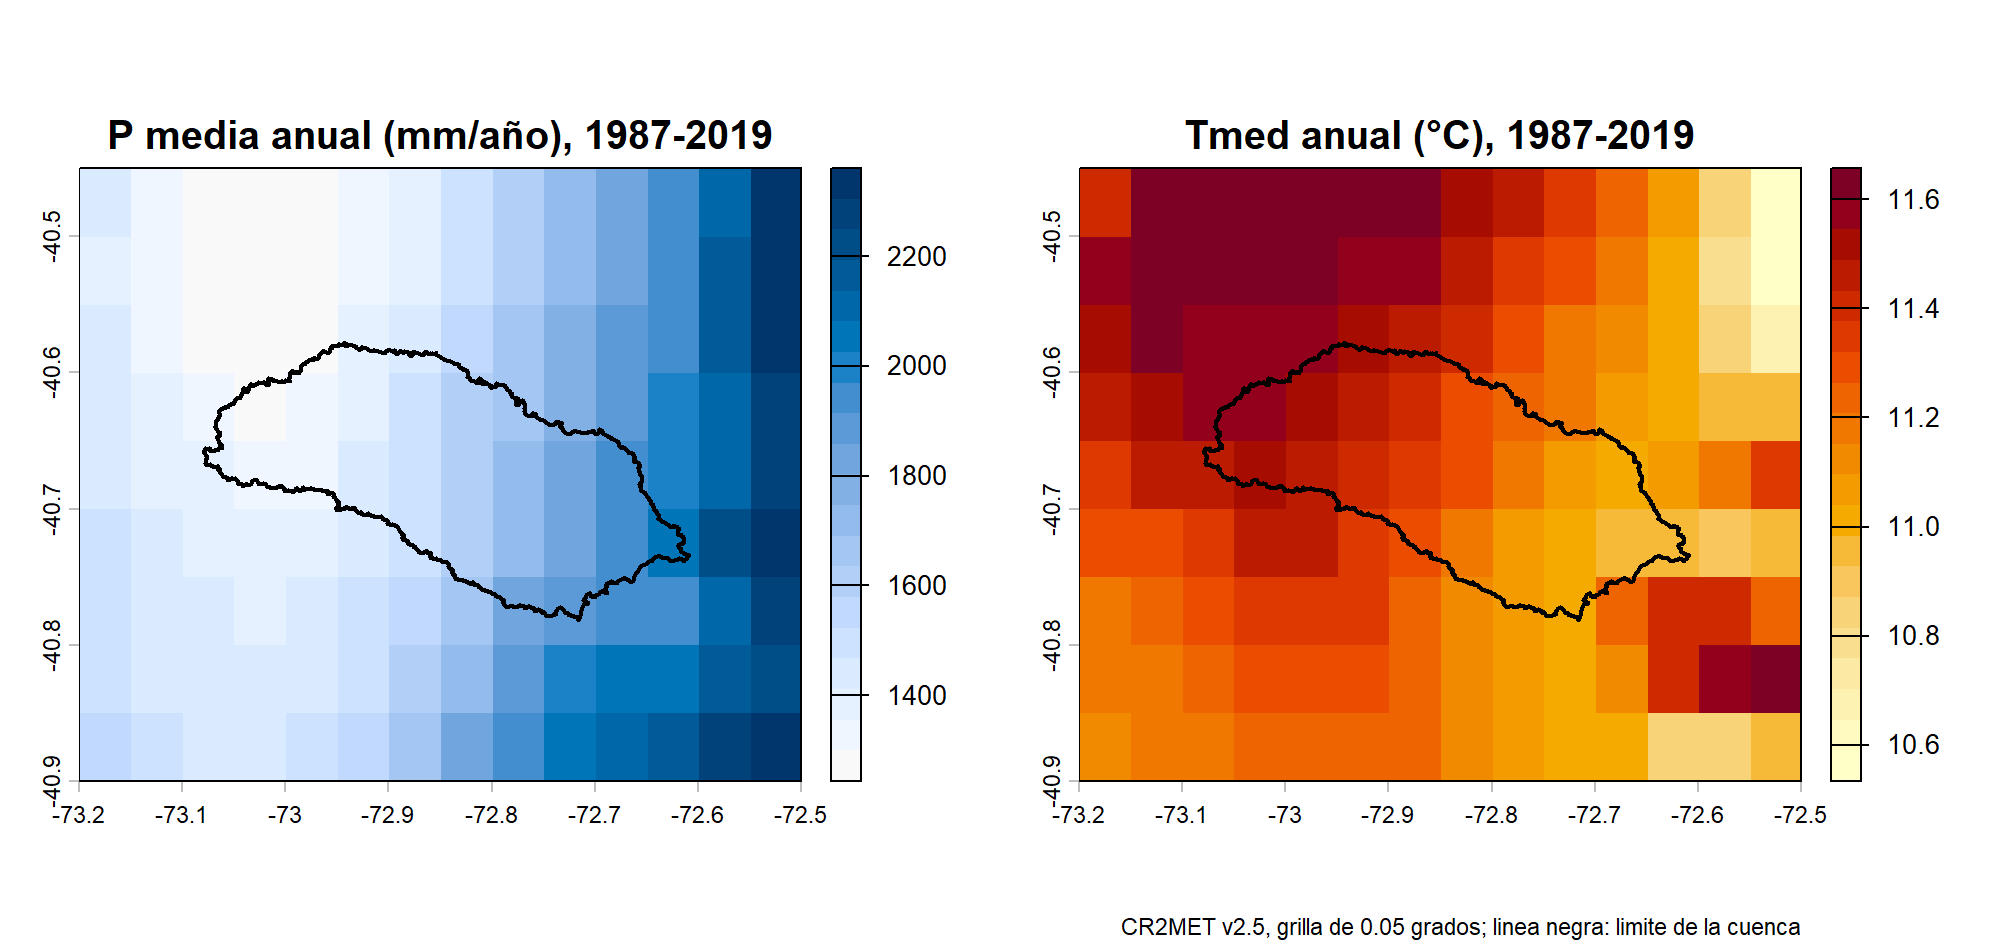
\includegraphics[width=0.95\textwidth]{../03_outputs/figures/05_mapas_P_T_media_anual.png}}{%
\fbox{Falta 03\_outputs/figures/05\_mapas\_P\_T\_media\_anual.png}}
\caption{P media anual (mm\,año$^{-1}$) y Tmed anual (°C) de CR2MET v2.5,
1987--2019, en la grilla de 0.05° (coordenadas geográficas WGS84,
EPSG:4326). La línea negra es el límite de la cuenca.}
\label{fig:E03mapas}
\end{figure}

\begin{figure}[ht]
\centering
\IfFileExists{../03_outputs/figures/05_mapa_koppen.png}{%
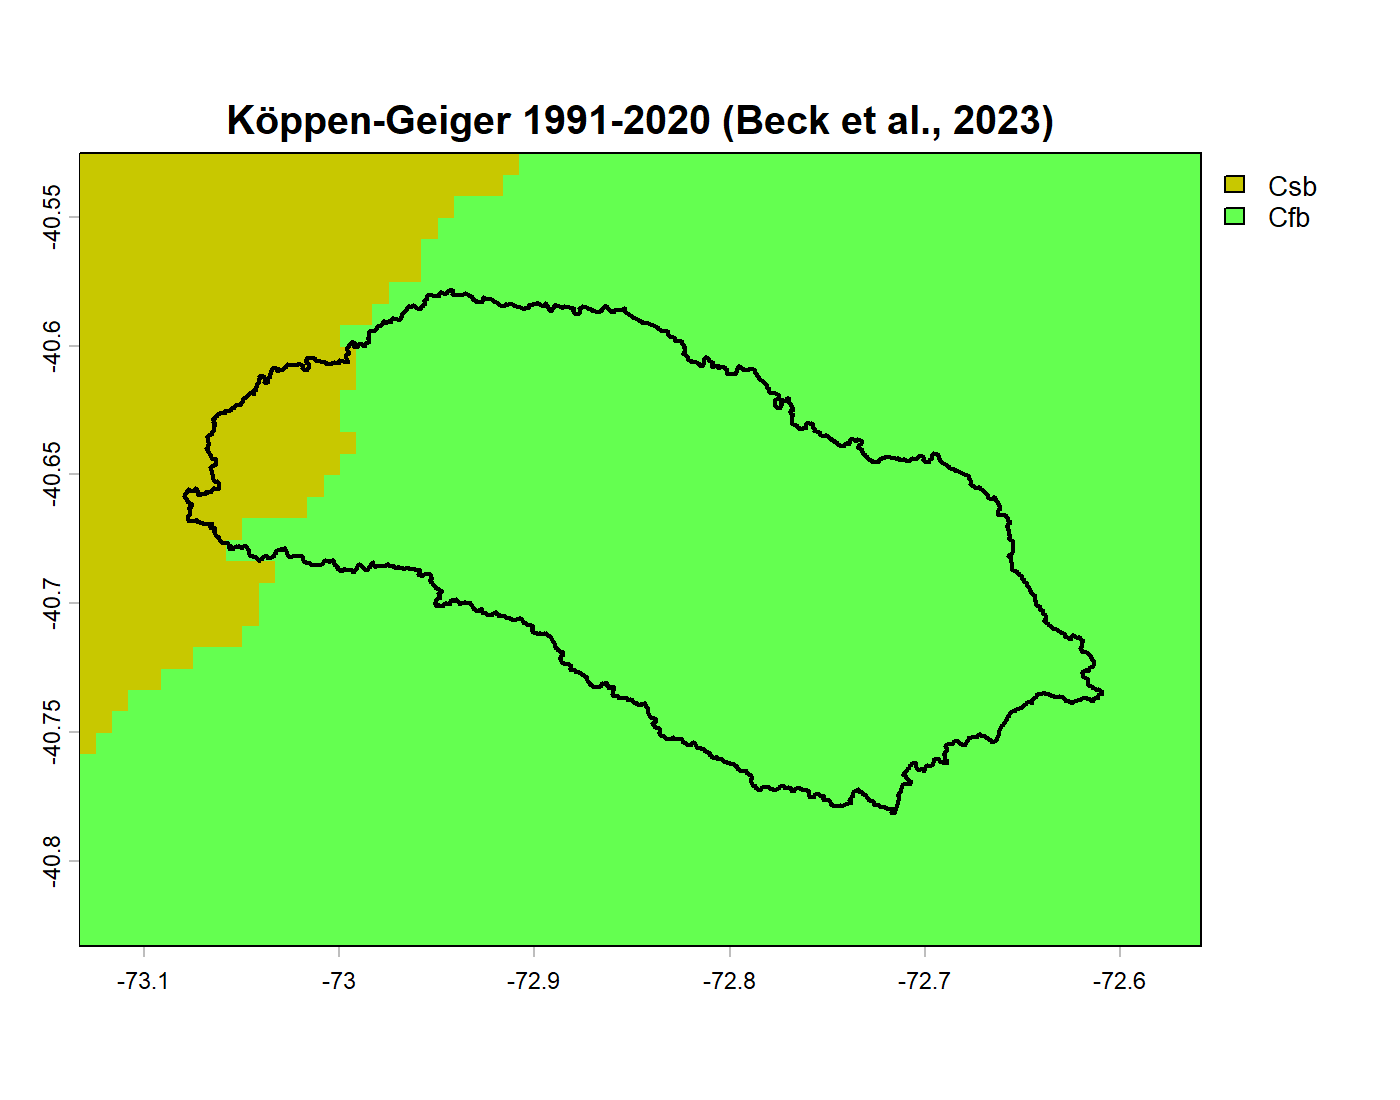
\includegraphics[width=0.7\textwidth]{../03_outputs/figures/05_mapa_koppen.png}}{%
\fbox{Falta 03\_outputs/figures/05\_mapa\_koppen.png}}
\caption{Clasificación de Köppen-Geiger 1991--2020 de \citet{Beck2023}, en
la grilla de 1 km (coordenadas geográficas WGS84). Cfb: templado, sin
estación seca y con verano templado. Csb: templado, con verano seco y
templado. La línea negra es el límite de la cuenca.}
\label{fig:E03koppen}
\end{figure}

\campo{3. Fuente y trazabilidad}{P, Tmax y Tmin vienen de CR2MET v2.5
\citep{Boisier2023} (grilla de 0.05°, WGS84) y la PET de
\citet{Hargreaves1985}, todo promediado sobre el polígono de la cuenca de E01
(ver E02). El caudal es la serie DGA rellenada por el integrante 2.
\texttt{02\_\allowbreak{}Rscripts/\allowbreak{}05\_\allowbreak{}regimen\_\allowbreak{}hidroclimatico.R} agrega a escala mensual
(P, PET y Q se suman, las temperaturas se promedian), promedia cada mes del
año en 1987--2019, recorta el mapa de Köppen-Geiger y escribe las cifras en
\texttt{03\_\allowbreak{}outputs/\allowbreak{}tables/\allowbreak{}} (\texttt{05\_\allowbreak{}climatologia\_\allowbreak{}mensual.csv},
\texttt{05\_\allowbreak{}regimen\_\allowbreak{}mensual\_\allowbreak{}P\_\allowbreak{}PET\_\allowbreak{}Q.csv},
\texttt{05\_\allowbreak{}resumen\_\allowbreak{}regimen\_\allowbreak{}E03.csv}, \texttt{05\_\allowbreak{}indice\_\allowbreak{}aridez.csv},
\texttt{05\_\allowbreak{}mapas\_\allowbreak{}rango\_\allowbreak{}en\_\allowbreak{}cuenca.csv} y \texttt{05\_\allowbreak{}koppen\_\allowbreak{}cuenca.csv}) y
las figuras en \texttt{03\_\allowbreak{}outputs/\allowbreak{}figures/\allowbreak{}} (\texttt{05\_\allowbreak{}climograma.png},
\texttt{05\_\allowbreak{}regimen\_\allowbreak{}P\_\allowbreak{}PET\_\allowbreak{}Q.png}, \texttt{05\_\allowbreak{}mapas\_\allowbreak{}P\_\allowbreak{}T\_\allowbreak{}media\_\allowbreak{}anual.png}
y \texttt{05\_\allowbreak{}mapa\_\allowbreak{}koppen.png}). Los mapas de P y T se rehacen solo donde
están las grillas de CR2MET; el de Köppen se rehace desde el recorte que
queda en \texttt{01\_\allowbreak{}data/\allowbreak{}processed/\allowbreak{}}. Las fuentes están en
\texttt{04\_\allowbreak{}metadata/\allowbreak{}data\_\allowbreak{}sources.csv}, el período en
\texttt{06\_\allowbreak{}config/\allowbreak{}parametros.csv}, y todo se regenera con
\texttt{run\_\allowbreak{}all.R}.}

\campo{4. Interpretación hidrológica}{El régimen es pluvial. La P se concentra
entre mayo y agosto (54.1 \% del año, máximo en junio) y el caudal la sigue
con uno o dos meses de retraso: el máximo es en julio y agosto, y entre mayo y
agosto pasa el 66.6 \% del caudal anual. No hay un segundo máximo en
primavera, que sería la señal de un aporte nival, y la cuenca es baja
(cotas bajo 350 m, E01). En septiembre el cociente Q/P sigue tan alto como en
agosto (0.55 y 0.56), lo que sugiere un almacenamiento que se vacía después
del invierno, aunque con esta evidencia no se puede decir dónde está (suelo,
acuífero o lagos).

En verano el clima pasa a estar limitado por agua: de noviembre a marzo la
PET supera a la P, el caudal cae a 6 mm\,mes$^{-1}$ en febrero y marzo y la
razón entre el mes de más caudal y el de menos es 19. A escala anual la
cuenca está limitada por energía, con PET/P = 0.608, menor que 1. La
clasificación de Köppen-Geiger es coherente con ese cuadro: el 92.6 \% del
área es Cfb (templado, sin estación seca) y solo el borde oeste, cerca de
Osorno, es Csb (con verano seco). La P de CR2MET aumenta de oeste a este
dentro de la cuenca, mientras la Tmed casi no varía.}

\campo{5. Consistencia física}{El índice de aridez usado es el cociente
PET/P del enfoque de Budyko \citep{Sposito2017}, el mismo de E06, y el
caudal en lámina sale de dividir el volumen por el área:
\begin{equation}
\phi = \frac{\mathrm{PET}}{P}, \qquad
c_Q = \frac{Q}{P}
\label{eq:E03aridez}
\end{equation}
\begin{equation}
Q_{\mathrm{mm/d}} = \frac{86{.}4\, Q_{\mathrm{m^3/s}}}{A_{\mathrm{km^2}}}
\label{eq:E03lamina}
\end{equation}
P, PET y Q se suman en el mes y las temperaturas se promedian; la fila anual
de la Tabla~\ref{tab:E03mensual} cierra con los totales. La PET es máxima en
enero y mínima en junio, como la radiación extraterrestre que usa la
ecuación de Hargreaves, y va un mes antes que la Tmed (máxima en febrero,
mínima en julio). Tmin queda siempre bajo Tmed y Tmed bajo Tmax. Hay una
inconsistencia que se arrastra a E06: la ET real que deja el balance,
(P $-$ Q)/P = 0.647, es mayor que PET/P = 0.608, así que el punto de la
cuenca queda sobre el límite de energía de Budyko (ver E04 y E06).}

\campo{6. Limitaciones e incertidumbre}{La P y la T son de un producto
grillado de 0.05° (unos 5 km) y no de estaciones dentro de la cuenca, así que
el gradiente de P hacia el este depende de cómo CR2MET reparte la lluvia; el
rango de la Tabla~\ref{tab:E03indices} incluye celdas que solo tocan el
borde de la cuenca. El caudal de 11 de los 33 años incluye días rellenados
(E02). Entre ellos hay 19 días de verano de 2014--2015 en 0 m$^3$\,s$^{-1}$,
que son un artefacto de la regresión y no un caudal observado. El rol del
almacenamiento en la recesión de primavera es una inferencia del desfase
entre P y Q, no una observación. El mapa de Köppen-Geiger es de 1991--2020 y
no de 1987--2019.}

\campo{7. Conclusión asociada}{En 1987--2019 la cuenca del Río Damas en
Tacamo tiene un régimen pluvial: la lluvia de otoño e invierno (máximo en
junio) produce el máximo de caudal en julio y agosto, y en verano la PET
supera a la P y el caudal baja a su mínimo. A escala anual la cuenca está
limitada por energía (PET/P = 0.608) y su clima es templado sin estación
seca (Cfb en el 92.6 \% del área).}

% Cifras: 03_outputs/tables/05_climatologia_mensual.csv, 05_regimen_mensual_P_PET_Q.csv,
% 05_resumen_regimen_E03.csv, 05_indice_aridez.csv, 05_mapas_rango_en_cuenca.csv,
% 05_koppen_cuenca.csv y 05_relaciones_anuales_E04.csv, generadas por run_all.R.
% Periodo 1987-2019, poligono de Alexis, caudal rellenado.

\section{E03. Régimen hidroclimático}
\label{ev:E03}

\campo{1. Pregunta o afirmación que se evalúa}{¿Qué estacionalidad y qué
procesos dominan el régimen de la cuenca?}

\campo{2. Evidencia principal}{El climograma (Figura~\ref{fig:E03climograma})
y el régimen mensual de P, PET y Q (Figura~\ref{fig:E03regimen}), con sus
valores en la Tabla~\ref{tab:E03mensual}. La Tabla~\ref{tab:E03indices}
resume los índices anuales, la Figura~\ref{fig:E03mapas} muestra la P y la
Tmed anuales en la grilla de CR2MET y la Figura~\ref{fig:E03koppen}, la
clasificación de Köppen-Geiger. Todo para 1987--2019: 33 años, 396 meses por
variable.}

\begin{figure}[ht]
\centering
\IfFileExists{../03_outputs/figures/05_climograma.png}{%
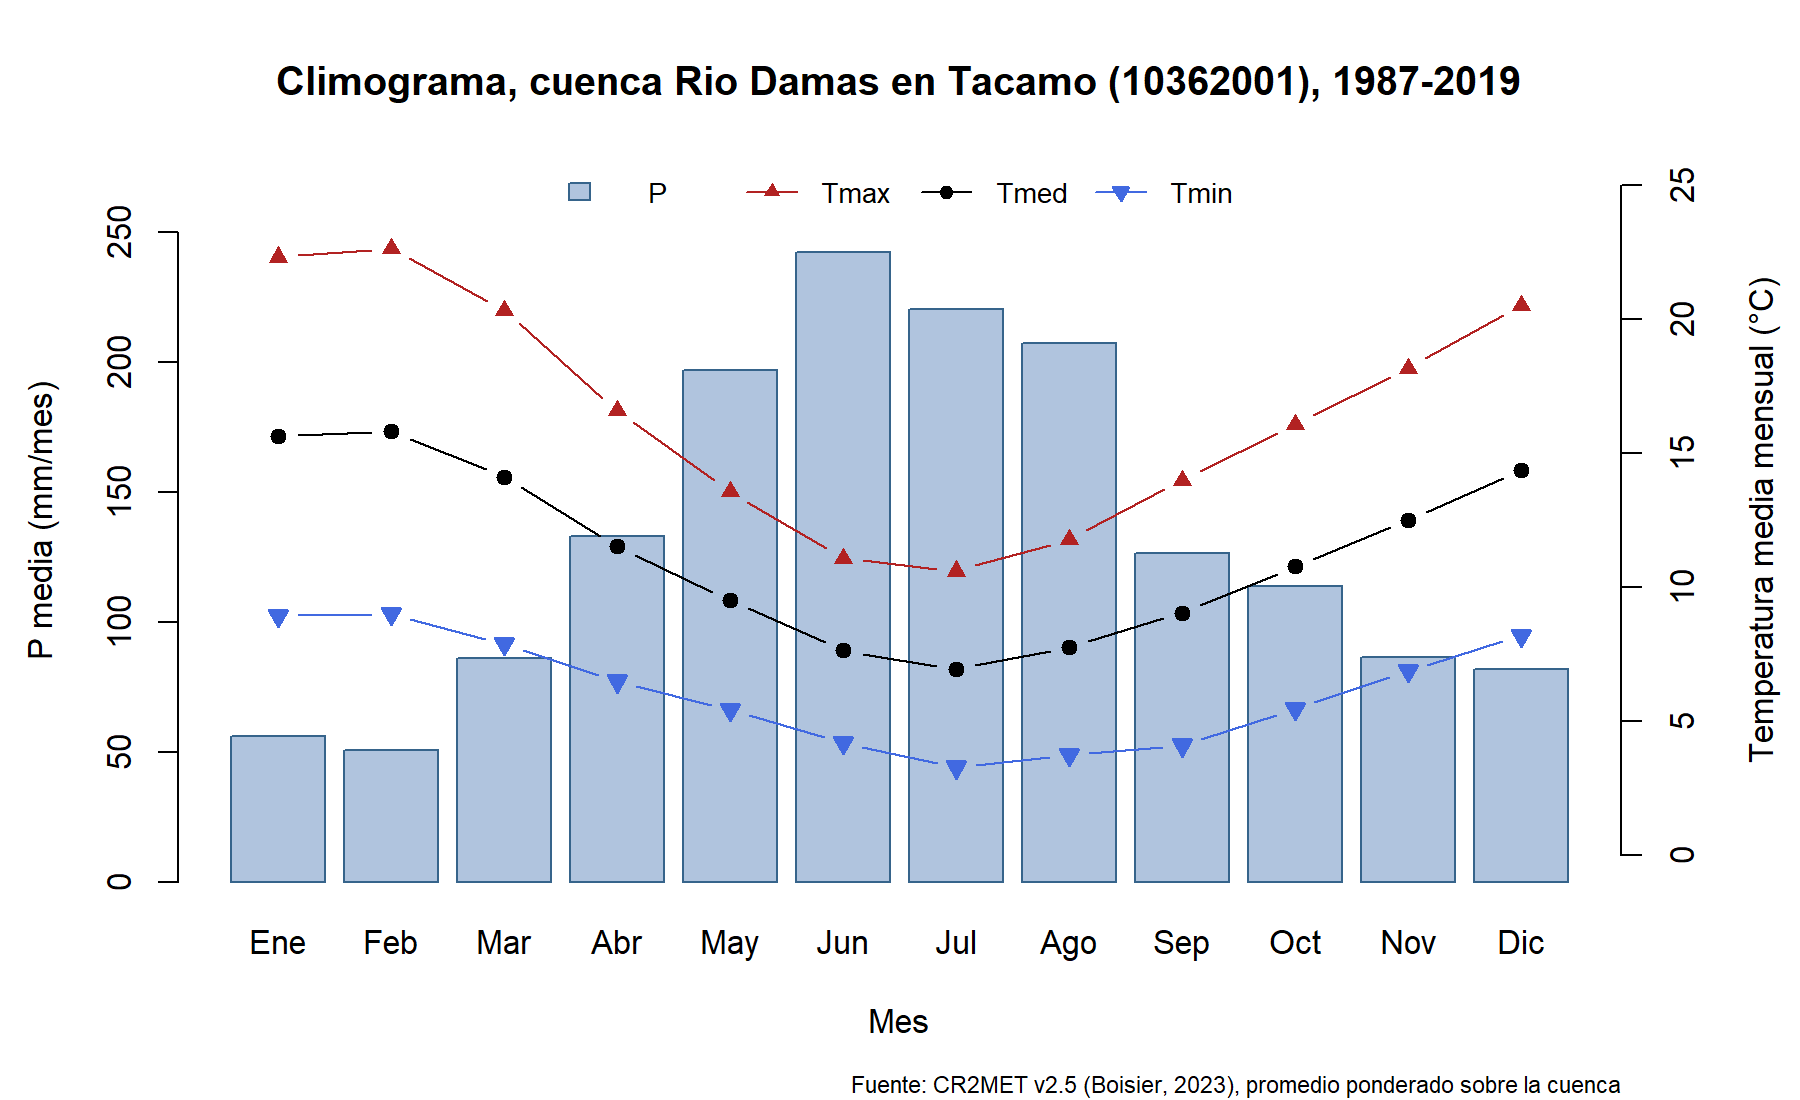
\includegraphics[width=0.85\textwidth]{../03_outputs/figures/05_climograma.png}}{%
\fbox{Falta 03\_outputs/figures/05\_climograma.png}}
\caption{Climograma de la cuenca, 1987--2019: P media mensual (barras,
mm\,mes$^{-1}$) y Tmax, Tmed y Tmin medias mensuales (líneas, °C), de CR2MET
v2.5 \citep{Boisier2023} promediado sobre la cuenca.}
\label{fig:E03climograma}
\end{figure}

\begin{figure}[ht]
\centering
\IfFileExists{../03_outputs/figures/05_regimen_P_PET_Q.png}{%
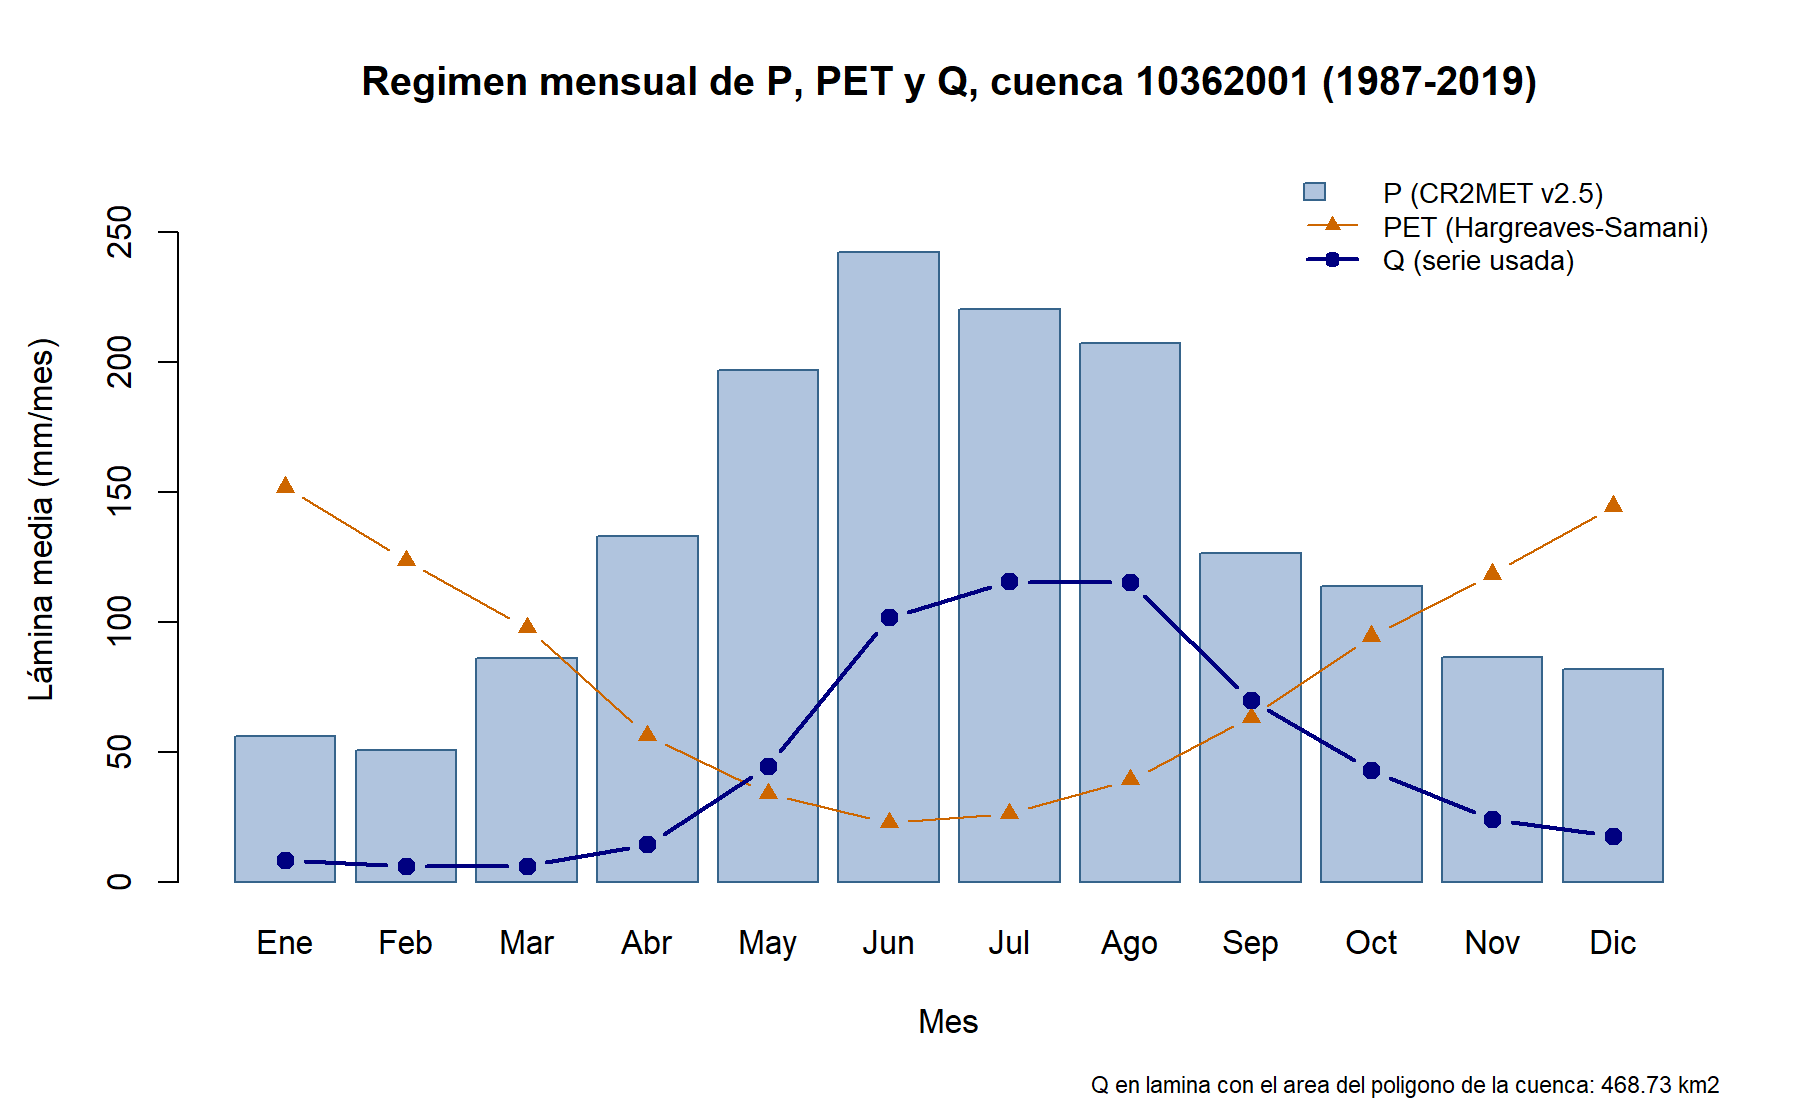
\includegraphics[width=0.85\textwidth]{../03_outputs/figures/05_regimen_P_PET_Q.png}}{%
\fbox{Falta 03\_outputs/figures/05\_regimen\_P\_PET\_Q.png}}
\caption{Régimen mensual de P, PET y Q en lámina (mm\,mes$^{-1}$),
1987--2019. Q es el caudal DGA rellenado por el integrante 2 (E02), pasado a
lámina con el área de la cuenca de E01 (468.73 km$^2$) según la
ecuación~(\ref{eq:E03lamina}).}
\label{fig:E03regimen}
\end{figure}

\begin{table}[ht]
\centering
\caption{Valores medios mensuales, 1987--2019 (33 años). P, PET y Q en
mm\,mes$^{-1}$; Q/P adimensional; temperaturas en °C. La fila del año suma
los valores sin redondear (P, PET y Q en mm\,año$^{-1}$) y da la media anual
de las temperaturas.}
\label{tab:E03mensual}
\begin{tabular}{|l|r|r|r|r|r|r|r|}
\hline
Mes & P & PET & Q & Q/P & Tmax & Tmed & Tmin \\
\hline
Ene & 56.3 & 152.0 & 8.3 & 0.15 & 22.31 & 15.61 & 8.92 \\
\hline
Feb & 50.6 & 123.8 & 6.0 & 0.12 & 22.63 & 15.81 & 9.00 \\
\hline
Mar & 86.2 & 98.0 & 6.2 & 0.07 & 20.32 & 14.10 & 7.87 \\
\hline
Abr & 133.1 & 56.4 & 14.4 & 0.11 & 16.57 & 11.52 & 6.48 \\
\hline
May & 196.8 & 34.0 & 44.4 & 0.23 & 13.55 & 9.49 & 5.43 \\
\hline
Jun & 242.3 & 22.9 & 101.7 & 0.42 & 11.07 & 7.63 & 4.18 \\
\hline
Jul & 220.5 & 26.2 & 115.6 & 0.52 & 10.60 & 6.93 & 3.27 \\
\hline
Ago & 207.3 & 39.3 & 115.4 & 0.56 & 11.77 & 7.76 & 3.75 \\
\hline
Sep & 126.5 & 63.3 & 69.8 & 0.55 & 13.98 & 9.04 & 4.10 \\
\hline
Oct & 113.8 & 94.6 & 42.8 & 0.38 & 16.07 & 10.76 & 5.45 \\
\hline
Nov & 86.5 & 118.4 & 24.1 & 0.28 & 18.16 & 12.51 & 6.87 \\
\hline
Dic & 81.9 & 144.6 & 17.5 & 0.21 & 20.49 & 14.34 & 8.18 \\
\hline
Año & 1601.6 & 973.4 & 566.1 & 0.35 & 16.43 & 11.27 & 6.11 \\
\hline
\end{tabular}
\end{table}

\begin{table}[ht]
\centering
\caption{Índices del período 1987--2019. Las razones son adimensionales.}
\label{tab:E03indices}
\begin{tabular}{|p{0.5\linewidth}|p{0.35\linewidth}|}
\hline
Indicador & Valor \\
\hline
P media anual & 1601.6 mm\,año$^{-1}$ \\
\hline
PET media anual \citep{Hargreaves1985} & 973.4 mm\,año$^{-1}$ \\
\hline
Q medio anual & 566.1 mm\,año$^{-1}$ (8.41 m$^3$\,s$^{-1}$) \\
\hline
Índice de aridez PET/P, ecuación~(\ref{eq:E03aridez}) & 0.608 \\
\hline
Coeficiente de escorrentía Q/P, ecuación~(\ref{eq:E03aridez}) & 0.353 \\
\hline
ET real por balance sobre P, (P $-$ Q)/P & 0.647 \\
\hline
P de mayo a agosto & 54.1 \% del año \\
\hline
Q de mayo a agosto & 66.6 \% del año \\
\hline
Meses con PET mayor que P & enero, febrero, marzo, noviembre y diciembre \\
\hline
P media anual en las celdas de 0.05° que tocan la cuenca & 1291.3 a 2034.4 mm\,año$^{-1}$ \\
\hline
Tmed anual en las celdas de 0.05° que tocan la cuenca & 10.9 a 11.6 °C \\
\hline
Köppen-Geiger 1991--2020 \citep{Beck2023}, \% del área & Cfb 92.6; Csb 7.4 \\
\hline
\end{tabular}
\end{table}

\begin{figure}[ht]
\centering
\IfFileExists{../03_outputs/figures/05_mapas_P_T_media_anual.png}{%
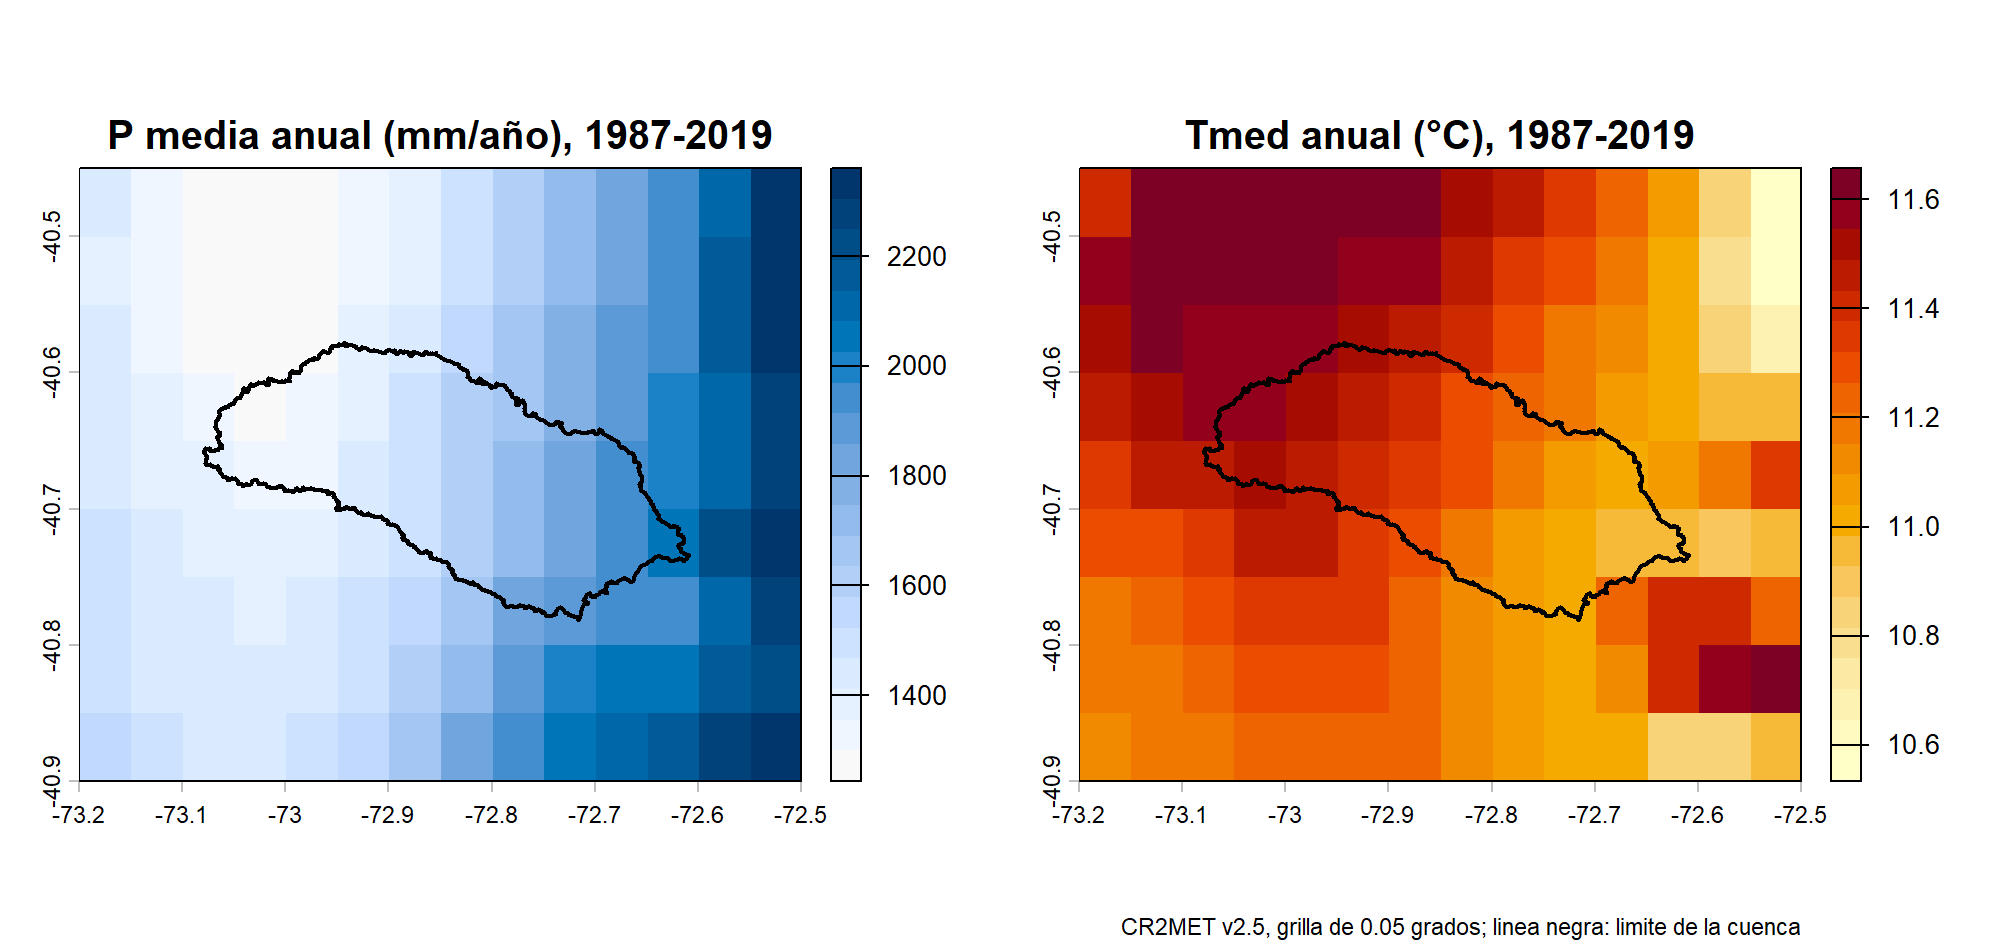
\includegraphics[width=0.95\textwidth]{../03_outputs/figures/05_mapas_P_T_media_anual.png}}{%
\fbox{Falta 03\_outputs/figures/05\_mapas\_P\_T\_media\_anual.png}}
\caption{P media anual (mm\,año$^{-1}$) y Tmed anual (°C) de CR2MET v2.5,
1987--2019, en la grilla de 0.05° (coordenadas geográficas WGS84,
EPSG:4326). La línea negra es el límite de la cuenca.}
\label{fig:E03mapas}
\end{figure}

\begin{figure}[ht]
\centering
\IfFileExists{../03_outputs/figures/05_mapa_koppen.png}{%
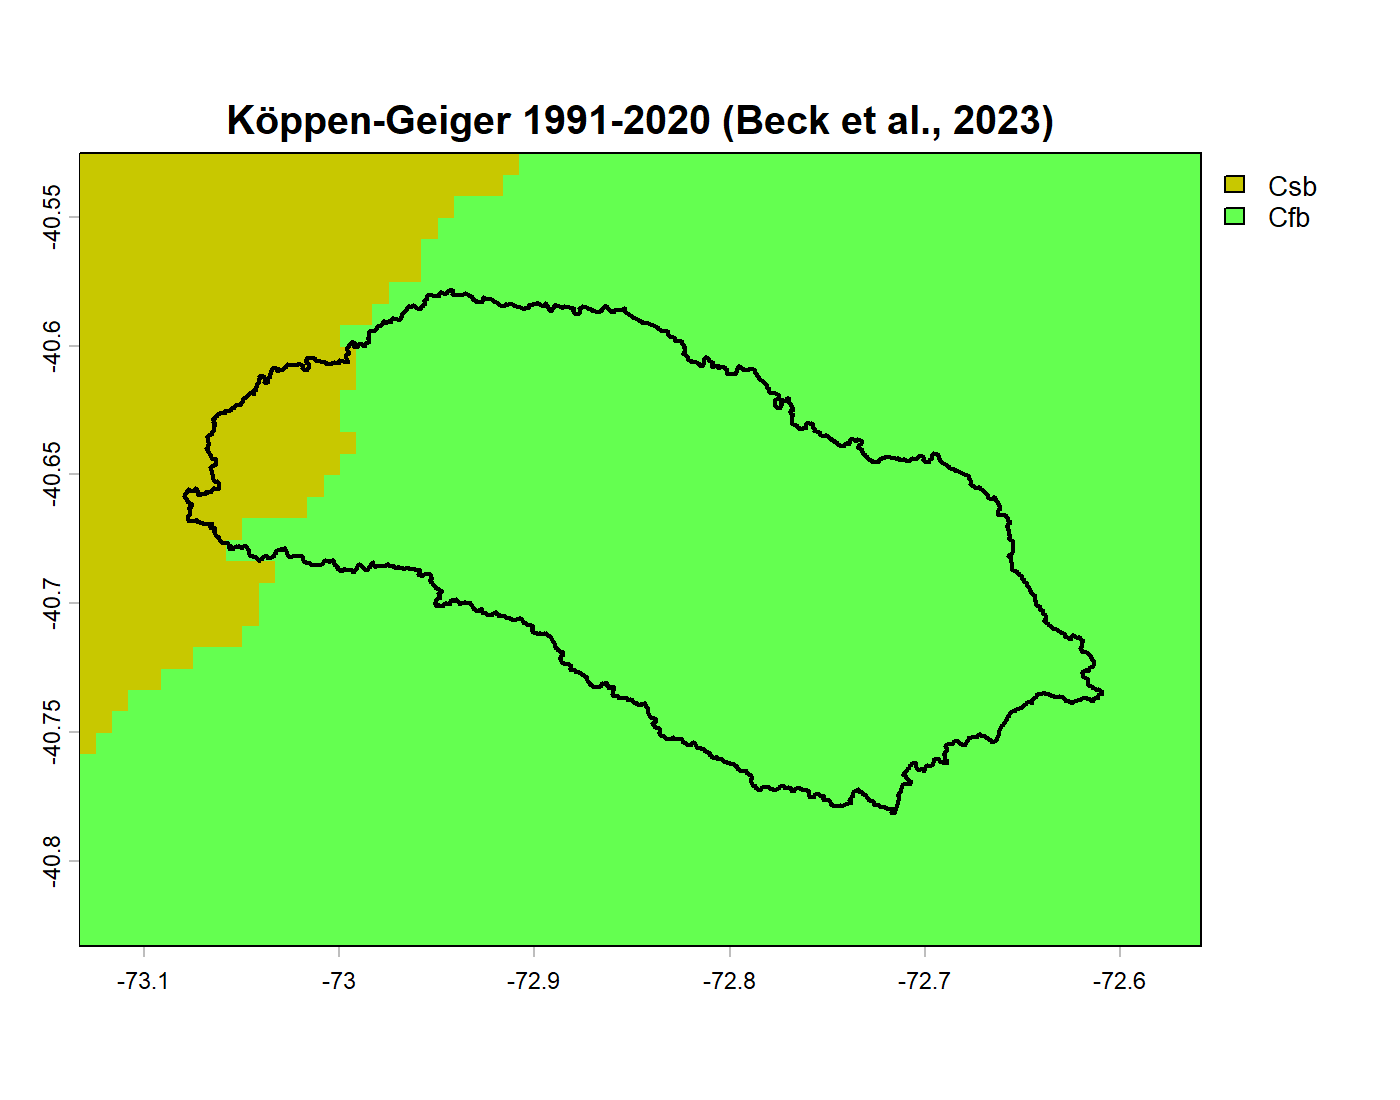
\includegraphics[width=0.7\textwidth]{../03_outputs/figures/05_mapa_koppen.png}}{%
\fbox{Falta 03\_outputs/figures/05\_mapa\_koppen.png}}
\caption{Clasificación de Köppen-Geiger 1991--2020 de \citet{Beck2023}, en
la grilla de 1 km (coordenadas geográficas WGS84). Cfb: templado, sin
estación seca y con verano templado. Csb: templado, con verano seco y
templado. La línea negra es el límite de la cuenca.}
\label{fig:E03koppen}
\end{figure}

\campo{3. Fuente y trazabilidad}{P, Tmax y Tmin vienen de CR2MET v2.5
\citep{Boisier2023} (grilla de 0.05°, WGS84) y la PET de
\citet{Hargreaves1985}, todo promediado sobre el polígono de la cuenca de E01
(ver E02). El caudal es la serie DGA rellenada por el integrante 2.
\texttt{02\_\allowbreak{}Rscripts/\allowbreak{}05\_\allowbreak{}regimen\_\allowbreak{}hidroclimatico.R} agrega a escala mensual
(P, PET y Q se suman, las temperaturas se promedian), promedia cada mes del
año en 1987--2019, recorta el mapa de Köppen-Geiger y escribe las cifras en
\texttt{03\_\allowbreak{}outputs/\allowbreak{}tables/\allowbreak{}} (\texttt{05\_\allowbreak{}climatologia\_\allowbreak{}mensual.csv},
\texttt{05\_\allowbreak{}regimen\_\allowbreak{}mensual\_\allowbreak{}P\_\allowbreak{}PET\_\allowbreak{}Q.csv},
\texttt{05\_\allowbreak{}resumen\_\allowbreak{}regimen\_\allowbreak{}E03.csv}, \texttt{05\_\allowbreak{}indice\_\allowbreak{}aridez.csv},
\texttt{05\_\allowbreak{}mapas\_\allowbreak{}rango\_\allowbreak{}en\_\allowbreak{}cuenca.csv} y \texttt{05\_\allowbreak{}koppen\_\allowbreak{}cuenca.csv}) y
las figuras en \texttt{03\_\allowbreak{}outputs/\allowbreak{}figures/\allowbreak{}} (\texttt{05\_\allowbreak{}climograma.png},
\texttt{05\_\allowbreak{}regimen\_\allowbreak{}P\_\allowbreak{}PET\_\allowbreak{}Q.png}, \texttt{05\_\allowbreak{}mapas\_\allowbreak{}P\_\allowbreak{}T\_\allowbreak{}media\_\allowbreak{}anual.png}
y \texttt{05\_\allowbreak{}mapa\_\allowbreak{}koppen.png}). Los mapas de P y T se rehacen solo donde
están las grillas de CR2MET; el de Köppen se rehace desde el recorte que
queda en \texttt{01\_\allowbreak{}data/\allowbreak{}processed/\allowbreak{}}. Las fuentes están en
\texttt{04\_\allowbreak{}metadata/\allowbreak{}data\_\allowbreak{}sources.csv}, el período en
\texttt{06\_\allowbreak{}config/\allowbreak{}parametros.csv}, y todo se regenera con
\texttt{run\_\allowbreak{}all.R}.}

\campo{4. Interpretación hidrológica}{El régimen es pluvial. La P se concentra
entre mayo y agosto (54.1 \% del año, máximo en junio) y el caudal la sigue
con uno o dos meses de retraso: el máximo es en julio y agosto, y entre mayo y
agosto pasa el 66.6 \% del caudal anual. No hay un segundo máximo en
primavera, que sería la señal de un aporte nival, y la cuenca es baja
(cotas bajo 350 m, E01). En septiembre el cociente Q/P sigue tan alto como en
agosto (0.55 y 0.56), lo que sugiere un almacenamiento que se vacía después
del invierno, aunque con esta evidencia no se puede decir dónde está (suelo,
acuífero o lagos).

En verano el clima pasa a estar limitado por agua: de noviembre a marzo la
PET supera a la P, el caudal cae a 6 mm\,mes$^{-1}$ en febrero y marzo y la
razón entre el mes de más caudal y el de menos es 19. A escala anual la
cuenca está limitada por energía, con PET/P = 0.608, menor que 1. La
clasificación de Köppen-Geiger es coherente con ese cuadro: el 92.6 \% del
área es Cfb (templado, sin estación seca) y solo el borde oeste, cerca de
Osorno, es Csb (con verano seco). La P de CR2MET aumenta de oeste a este
dentro de la cuenca, mientras la Tmed casi no varía.}

\campo{5. Consistencia física}{El índice de aridez usado es el cociente
PET/P del enfoque de Budyko \citep{Sposito2017}, el mismo de E06, y el
caudal en lámina sale de dividir el volumen por el área:
\begin{equation}
\phi = \frac{\mathrm{PET}}{P}, \qquad
c_Q = \frac{Q}{P}
\label{eq:E03aridez}
\end{equation}
\begin{equation}
Q_{\mathrm{mm/d}} = \frac{86{.}4\, Q_{\mathrm{m^3/s}}}{A_{\mathrm{km^2}}}
\label{eq:E03lamina}
\end{equation}
P, PET y Q se suman en el mes y las temperaturas se promedian; la fila anual
de la Tabla~\ref{tab:E03mensual} cierra con los totales. La PET es máxima en
enero y mínima en junio, como la radiación extraterrestre que usa la
ecuación de Hargreaves, y va un mes antes que la Tmed (máxima en febrero,
mínima en julio). Tmin queda siempre bajo Tmed y Tmed bajo Tmax. Hay una
inconsistencia que se arrastra a E06: la ET real que deja el balance,
(P $-$ Q)/P = 0.647, es mayor que PET/P = 0.608, así que el punto de la
cuenca queda sobre el límite de energía de Budyko (ver E04 y E06).}

\campo{6. Limitaciones e incertidumbre}{La P y la T son de un producto
grillado de 0.05° (unos 5 km) y no de estaciones dentro de la cuenca, así que
el gradiente de P hacia el este depende de cómo CR2MET reparte la lluvia; el
rango de la Tabla~\ref{tab:E03indices} incluye celdas que solo tocan el
borde de la cuenca. El caudal de 11 de los 33 años incluye días rellenados
(E02). Entre ellos hay 19 días de verano de 2014--2015 en 0 m$^3$\,s$^{-1}$,
que son un artefacto de la regresión y no un caudal observado. El rol del
almacenamiento en la recesión de primavera es una inferencia del desfase
entre P y Q, no una observación. El mapa de Köppen-Geiger es de 1991--2020 y
no de 1987--2019.}

\campo{7. Conclusión asociada}{En 1987--2019 la cuenca del Río Damas en
Tacamo tiene un régimen pluvial: la lluvia de otoño e invierno (máximo en
junio) produce el máximo de caudal en julio y agosto, y en verano la PET
supera a la P y el caudal baja a su mínimo. A escala anual la cuenca está
limitada por energía (PET/P = 0.608) y su clima es templado sin estación
seca (Cfb en el 92.6 \% del área).}

% Cifras: 03_outputs/tables/05_climatologia_mensual.csv, 05_regimen_mensual_P_PET_Q.csv,
% 05_resumen_regimen_E03.csv, 05_indice_aridez.csv, 05_mapas_rango_en_cuenca.csv,
% 05_koppen_cuenca.csv y 05_relaciones_anuales_E04.csv, generadas por run_all.R.
% Periodo 1987-2019, poligono de Alexis, caudal rellenado.

\section{E03. Régimen hidroclimático}
\label{ev:E03}

\campo{1. Pregunta o afirmación que se evalúa}{¿Qué estacionalidad y qué
procesos dominan el régimen de la cuenca?}

\campo{2. Evidencia principal}{El climograma (Figura~\ref{fig:E03climograma})
y el régimen mensual de P, PET y Q (Figura~\ref{fig:E03regimen}), con sus
valores en la Tabla~\ref{tab:E03mensual}. La Tabla~\ref{tab:E03indices}
resume los índices anuales, la Figura~\ref{fig:E03mapas} muestra la P y la
Tmed anuales en la grilla de CR2MET y la Figura~\ref{fig:E03koppen}, la
clasificación de Köppen-Geiger. Todo para 1987--2019: 33 años, 396 meses por
variable.}

\begin{figure}[ht]
\centering
\IfFileExists{../03_outputs/figures/05_climograma.png}{%
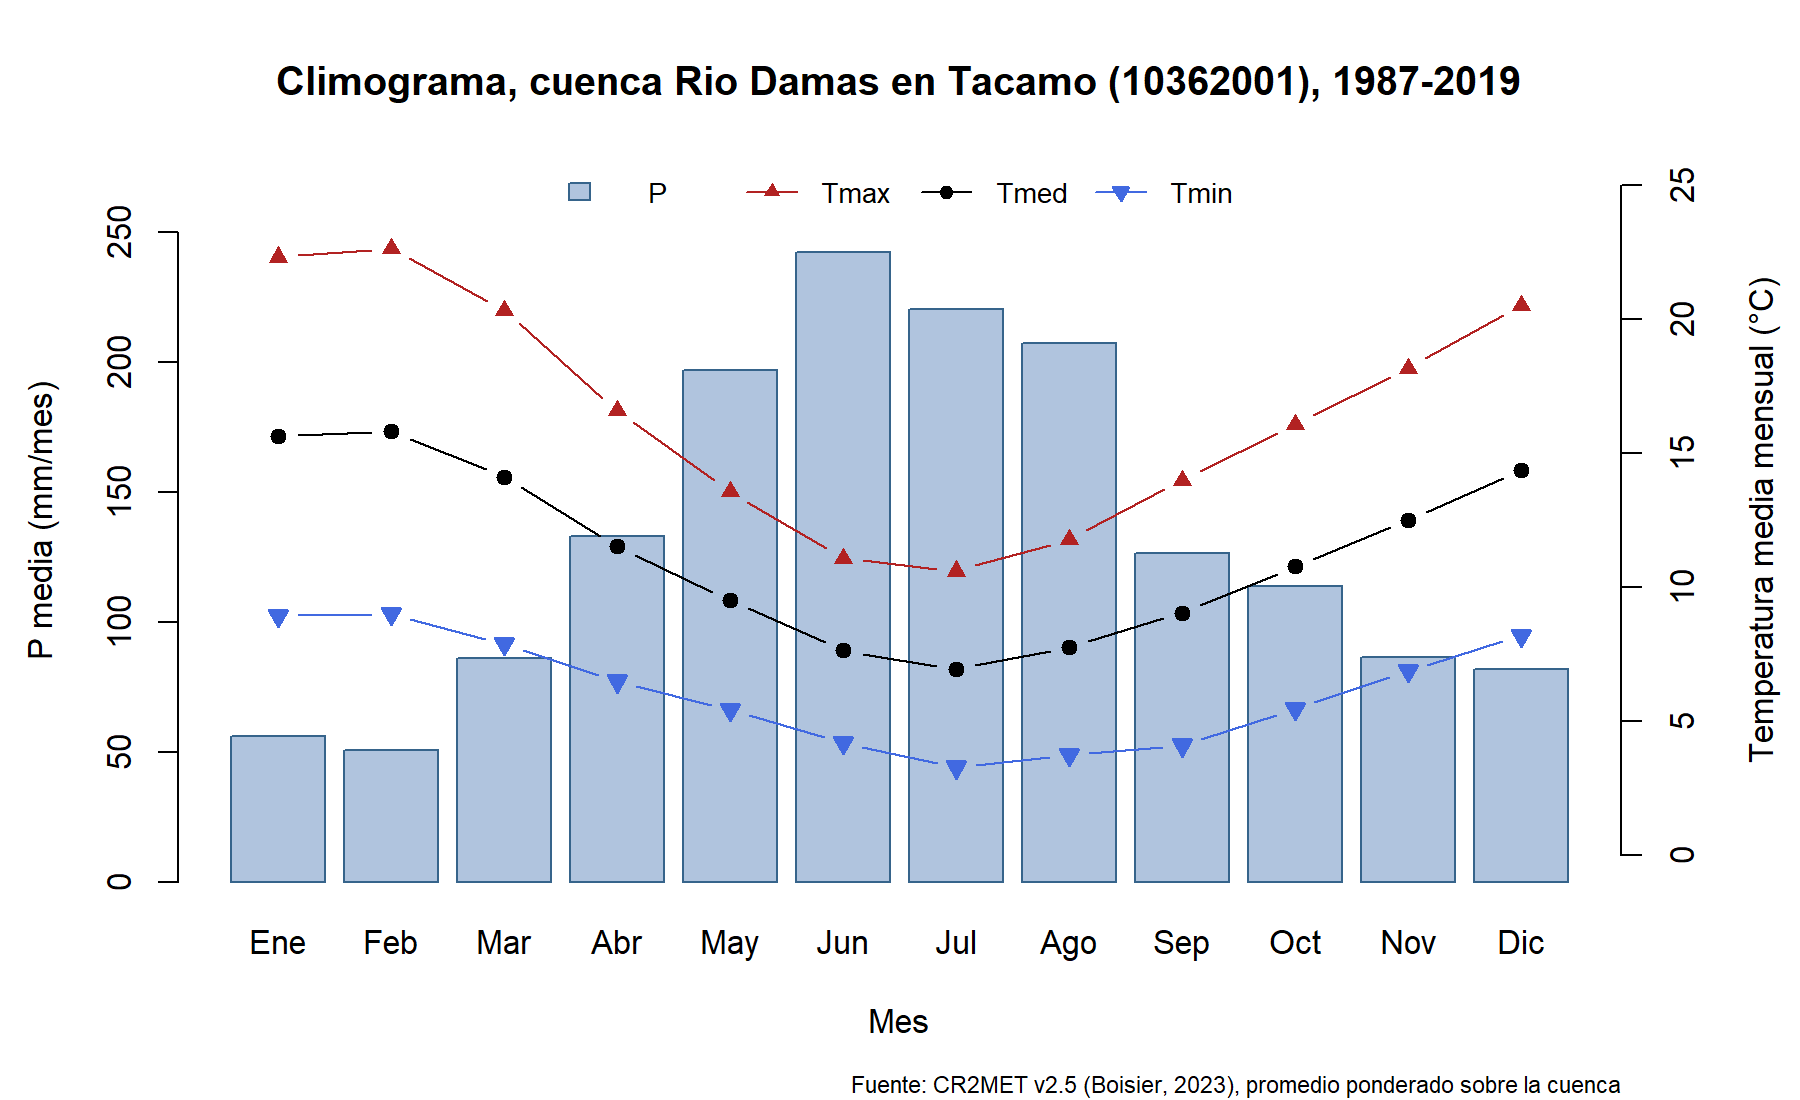
\includegraphics[width=0.85\textwidth]{../03_outputs/figures/05_climograma.png}}{%
\fbox{Falta 03\_outputs/figures/05\_climograma.png}}
\caption{Climograma de la cuenca, 1987--2019: P media mensual (barras,
mm\,mes$^{-1}$) y Tmax, Tmed y Tmin medias mensuales (líneas, °C), de CR2MET
v2.5 \citep{Boisier2023} promediado sobre la cuenca.}
\label{fig:E03climograma}
\end{figure}

\begin{figure}[ht]
\centering
\IfFileExists{../03_outputs/figures/05_regimen_P_PET_Q.png}{%
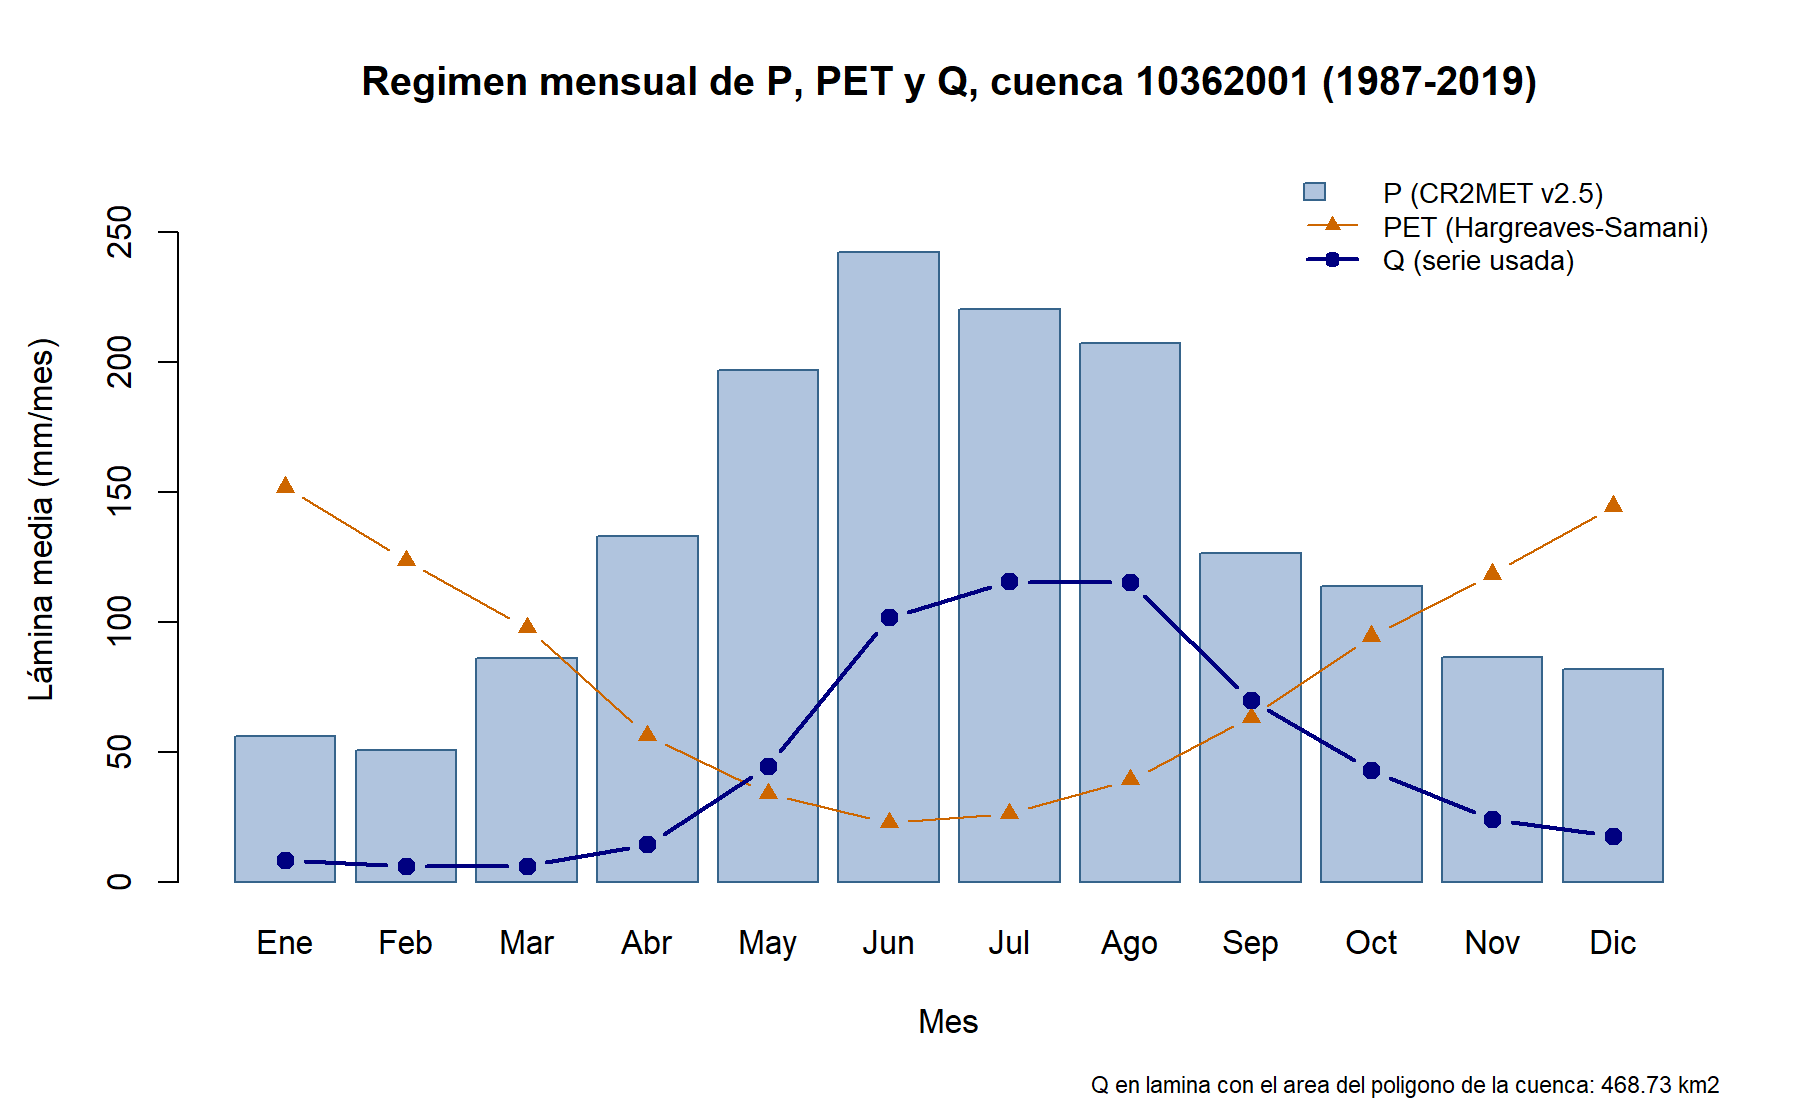
\includegraphics[width=0.85\textwidth]{../03_outputs/figures/05_regimen_P_PET_Q.png}}{%
\fbox{Falta 03\_outputs/figures/05\_regimen\_P\_PET\_Q.png}}
\caption{Régimen mensual de P, PET y Q en lámina (mm\,mes$^{-1}$),
1987--2019. Q es el caudal DGA rellenado por el integrante 2 (E02), pasado a
lámina con el área de la cuenca de E01 (468.73 km$^2$) según la
ecuación~(\ref{eq:E03lamina}).}
\label{fig:E03regimen}
\end{figure}

\begin{table}[ht]
\centering
\caption{Valores medios mensuales, 1987--2019 (33 años). P, PET y Q en
mm\,mes$^{-1}$; Q/P adimensional; temperaturas en °C. La fila del año suma
los valores sin redondear (P, PET y Q en mm\,año$^{-1}$) y da la media anual
de las temperaturas.}
\label{tab:E03mensual}
\begin{tabular}{|l|r|r|r|r|r|r|r|}
\hline
Mes & P & PET & Q & Q/P & Tmax & Tmed & Tmin \\
\hline
Ene & 56.3 & 152.0 & 8.3 & 0.15 & 22.31 & 15.61 & 8.92 \\
\hline
Feb & 50.6 & 123.8 & 6.0 & 0.12 & 22.63 & 15.81 & 9.00 \\
\hline
Mar & 86.2 & 98.0 & 6.2 & 0.07 & 20.32 & 14.10 & 7.87 \\
\hline
Abr & 133.1 & 56.4 & 14.4 & 0.11 & 16.57 & 11.52 & 6.48 \\
\hline
May & 196.8 & 34.0 & 44.4 & 0.23 & 13.55 & 9.49 & 5.43 \\
\hline
Jun & 242.3 & 22.9 & 101.7 & 0.42 & 11.07 & 7.63 & 4.18 \\
\hline
Jul & 220.5 & 26.2 & 115.6 & 0.52 & 10.60 & 6.93 & 3.27 \\
\hline
Ago & 207.3 & 39.3 & 115.4 & 0.56 & 11.77 & 7.76 & 3.75 \\
\hline
Sep & 126.5 & 63.3 & 69.8 & 0.55 & 13.98 & 9.04 & 4.10 \\
\hline
Oct & 113.8 & 94.6 & 42.8 & 0.38 & 16.07 & 10.76 & 5.45 \\
\hline
Nov & 86.5 & 118.4 & 24.1 & 0.28 & 18.16 & 12.51 & 6.87 \\
\hline
Dic & 81.9 & 144.6 & 17.5 & 0.21 & 20.49 & 14.34 & 8.18 \\
\hline
Año & 1601.6 & 973.4 & 566.1 & 0.35 & 16.43 & 11.27 & 6.11 \\
\hline
\end{tabular}
\end{table}

\begin{table}[ht]
\centering
\caption{Índices del período 1987--2019. Las razones son adimensionales.}
\label{tab:E03indices}
\begin{tabular}{|p{0.5\linewidth}|p{0.35\linewidth}|}
\hline
Indicador & Valor \\
\hline
P media anual & 1601.6 mm\,año$^{-1}$ \\
\hline
PET media anual \citep{Hargreaves1985} & 973.4 mm\,año$^{-1}$ \\
\hline
Q medio anual & 566.1 mm\,año$^{-1}$ (8.41 m$^3$\,s$^{-1}$) \\
\hline
Índice de aridez PET/P, ecuación~(\ref{eq:E03aridez}) & 0.608 \\
\hline
Coeficiente de escorrentía Q/P, ecuación~(\ref{eq:E03aridez}) & 0.353 \\
\hline
ET real por balance sobre P, (P $-$ Q)/P & 0.647 \\
\hline
P de mayo a agosto & 54.1 \% del año \\
\hline
Q de mayo a agosto & 66.6 \% del año \\
\hline
Meses con PET mayor que P & enero, febrero, marzo, noviembre y diciembre \\
\hline
P media anual en las celdas de 0.05° que tocan la cuenca & 1291.3 a 2034.4 mm\,año$^{-1}$ \\
\hline
Tmed anual en las celdas de 0.05° que tocan la cuenca & 10.9 a 11.6 °C \\
\hline
Köppen-Geiger 1991--2020 \citep{Beck2023}, \% del área & Cfb 92.6; Csb 7.4 \\
\hline
\end{tabular}
\end{table}

\begin{figure}[ht]
\centering
\IfFileExists{../03_outputs/figures/05_mapas_P_T_media_anual.png}{%
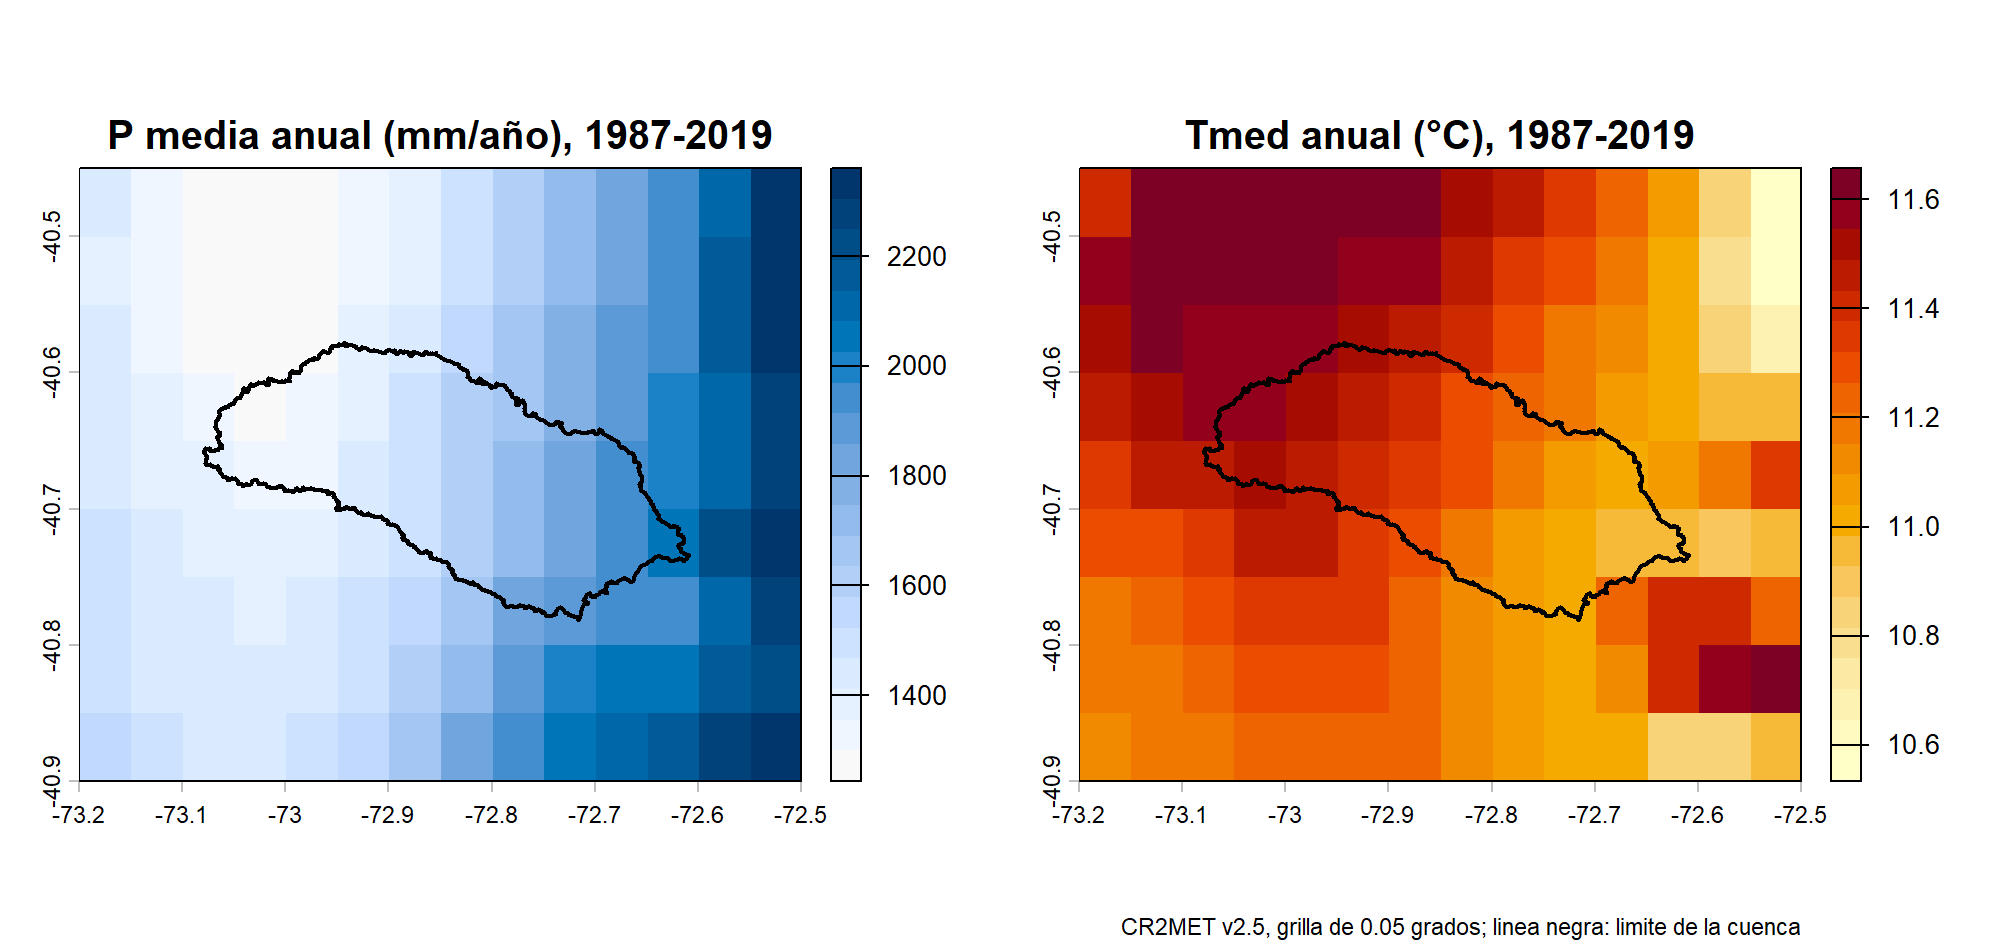
\includegraphics[width=0.95\textwidth]{../03_outputs/figures/05_mapas_P_T_media_anual.png}}{%
\fbox{Falta 03\_outputs/figures/05\_mapas\_P\_T\_media\_anual.png}}
\caption{P media anual (mm\,año$^{-1}$) y Tmed anual (°C) de CR2MET v2.5,
1987--2019, en la grilla de 0.05° (coordenadas geográficas WGS84,
EPSG:4326). La línea negra es el límite de la cuenca.}
\label{fig:E03mapas}
\end{figure}

\begin{figure}[ht]
\centering
\IfFileExists{../03_outputs/figures/05_mapa_koppen.png}{%
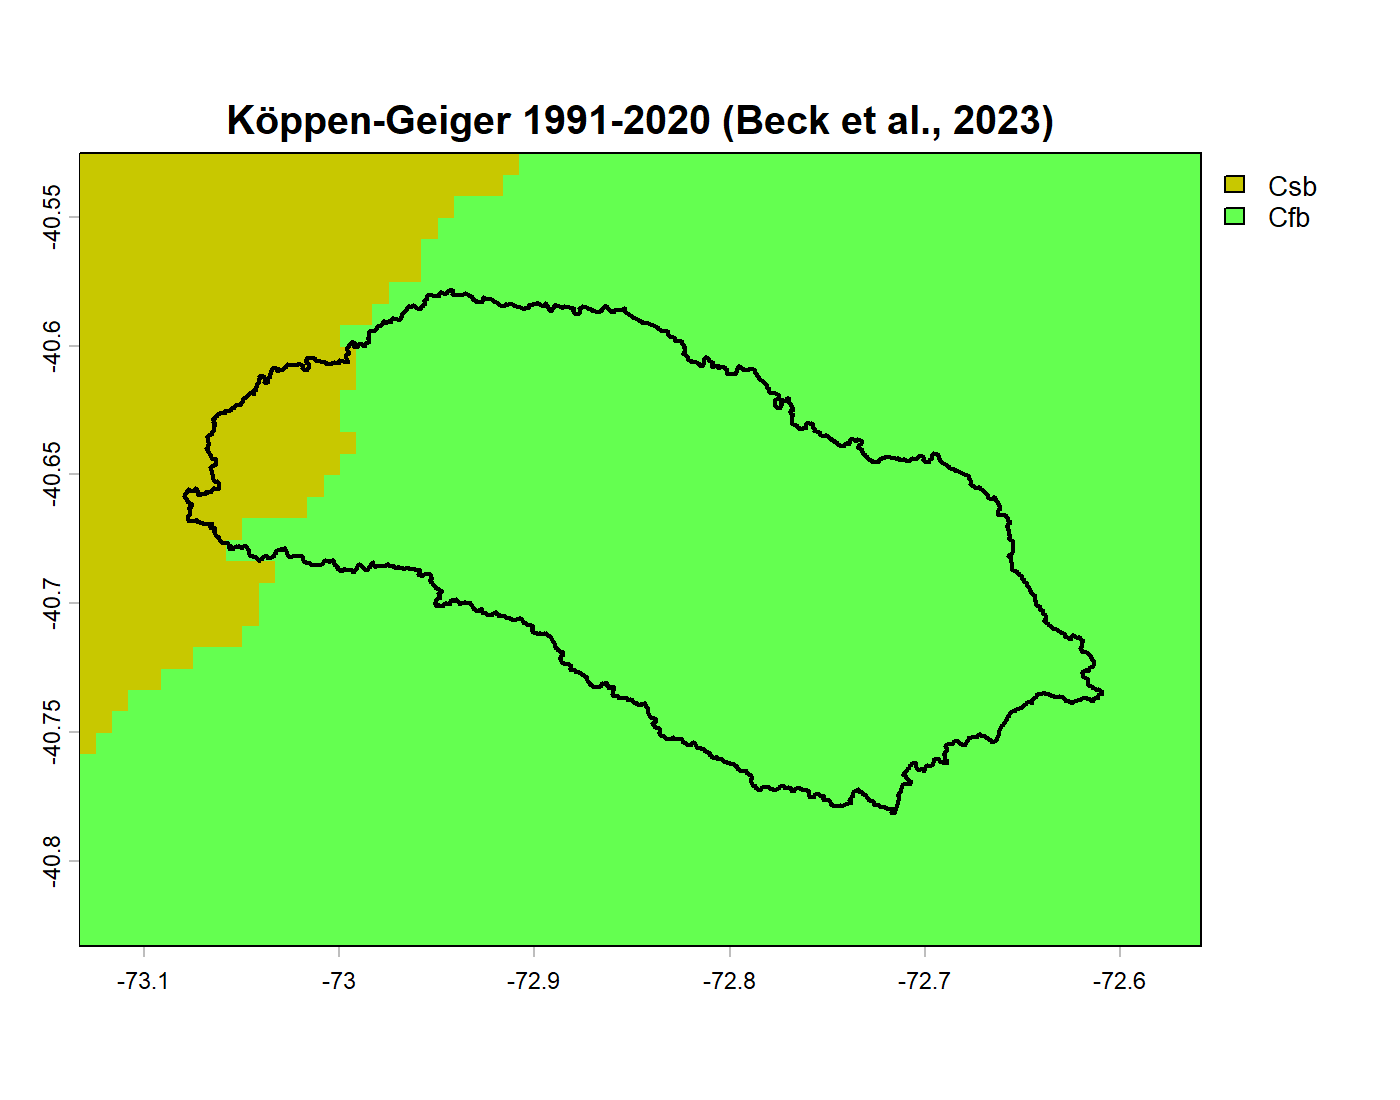
\includegraphics[width=0.7\textwidth]{../03_outputs/figures/05_mapa_koppen.png}}{%
\fbox{Falta 03\_outputs/figures/05\_mapa\_koppen.png}}
\caption{Clasificación de Köppen-Geiger 1991--2020 de \citet{Beck2023}, en
la grilla de 1 km (coordenadas geográficas WGS84). Cfb: templado, sin
estación seca y con verano templado. Csb: templado, con verano seco y
templado. La línea negra es el límite de la cuenca.}
\label{fig:E03koppen}
\end{figure}

\campo{3. Fuente y trazabilidad}{P, Tmax y Tmin vienen de CR2MET v2.5
\citep{Boisier2023} (grilla de 0.05°, WGS84) y la PET de
\citet{Hargreaves1985}, todo promediado sobre el polígono de la cuenca de E01
(ver E02). El caudal es la serie DGA rellenada por el integrante 2.
\texttt{02\_\allowbreak{}Rscripts/\allowbreak{}05\_\allowbreak{}regimen\_\allowbreak{}hidroclimatico.R} agrega a escala mensual
(P, PET y Q se suman, las temperaturas se promedian), promedia cada mes del
año en 1987--2019, recorta el mapa de Köppen-Geiger y escribe las cifras en
\texttt{03\_\allowbreak{}outputs/\allowbreak{}tables/\allowbreak{}} (\texttt{05\_\allowbreak{}climatologia\_\allowbreak{}mensual.csv},
\texttt{05\_\allowbreak{}regimen\_\allowbreak{}mensual\_\allowbreak{}P\_\allowbreak{}PET\_\allowbreak{}Q.csv},
\texttt{05\_\allowbreak{}resumen\_\allowbreak{}regimen\_\allowbreak{}E03.csv}, \texttt{05\_\allowbreak{}indice\_\allowbreak{}aridez.csv},
\texttt{05\_\allowbreak{}mapas\_\allowbreak{}rango\_\allowbreak{}en\_\allowbreak{}cuenca.csv} y \texttt{05\_\allowbreak{}koppen\_\allowbreak{}cuenca.csv}) y
las figuras en \texttt{03\_\allowbreak{}outputs/\allowbreak{}figures/\allowbreak{}} (\texttt{05\_\allowbreak{}climograma.png},
\texttt{05\_\allowbreak{}regimen\_\allowbreak{}P\_\allowbreak{}PET\_\allowbreak{}Q.png}, \texttt{05\_\allowbreak{}mapas\_\allowbreak{}P\_\allowbreak{}T\_\allowbreak{}media\_\allowbreak{}anual.png}
y \texttt{05\_\allowbreak{}mapa\_\allowbreak{}koppen.png}). Los mapas de P y T se rehacen solo donde
están las grillas de CR2MET; el de Köppen se rehace desde el recorte que
queda en \texttt{01\_\allowbreak{}data/\allowbreak{}processed/\allowbreak{}}. Las fuentes están en
\texttt{04\_\allowbreak{}metadata/\allowbreak{}data\_\allowbreak{}sources.csv}, el período en
\texttt{06\_\allowbreak{}config/\allowbreak{}parametros.csv}, y todo se regenera con
\texttt{run\_\allowbreak{}all.R}.}

\campo{4. Interpretación hidrológica}{El régimen es pluvial. La P se concentra
entre mayo y agosto (54.1 \% del año, máximo en junio) y el caudal la sigue
con uno o dos meses de retraso: el máximo es en julio y agosto, y entre mayo y
agosto pasa el 66.6 \% del caudal anual. No hay un segundo máximo en
primavera, que sería la señal de un aporte nival, y la cuenca es baja
(cotas bajo 350 m, E01). En septiembre el cociente Q/P sigue tan alto como en
agosto (0.55 y 0.56), lo que sugiere un almacenamiento que se vacía después
del invierno, aunque con esta evidencia no se puede decir dónde está (suelo,
acuífero o lagos).

En verano el clima pasa a estar limitado por agua: de noviembre a marzo la
PET supera a la P, el caudal cae a 6 mm\,mes$^{-1}$ en febrero y marzo y la
razón entre el mes de más caudal y el de menos es 19. A escala anual la
cuenca está limitada por energía, con PET/P = 0.608, menor que 1. La
clasificación de Köppen-Geiger es coherente con ese cuadro: el 92.6 \% del
área es Cfb (templado, sin estación seca) y solo el borde oeste, cerca de
Osorno, es Csb (con verano seco). La P de CR2MET aumenta de oeste a este
dentro de la cuenca, mientras la Tmed casi no varía.}

\campo{5. Consistencia física}{El índice de aridez usado es el cociente
PET/P del enfoque de Budyko \citep{Sposito2017}, el mismo de E06, y el
caudal en lámina sale de dividir el volumen por el área:
\begin{equation}
\phi = \frac{\mathrm{PET}}{P}, \qquad
c_Q = \frac{Q}{P}
\label{eq:E03aridez}
\end{equation}
\begin{equation}
Q_{\mathrm{mm/d}} = \frac{86{.}4\, Q_{\mathrm{m^3/s}}}{A_{\mathrm{km^2}}}
\label{eq:E03lamina}
\end{equation}
P, PET y Q se suman en el mes y las temperaturas se promedian; la fila anual
de la Tabla~\ref{tab:E03mensual} cierra con los totales. La PET es máxima en
enero y mínima en junio, como la radiación extraterrestre que usa la
ecuación de Hargreaves, y va un mes antes que la Tmed (máxima en febrero,
mínima en julio). Tmin queda siempre bajo Tmed y Tmed bajo Tmax. Hay una
inconsistencia que se arrastra a E06: la ET real que deja el balance,
(P $-$ Q)/P = 0.647, es mayor que PET/P = 0.608, así que el punto de la
cuenca queda sobre el límite de energía de Budyko (ver E04 y E06).}

\campo{6. Limitaciones e incertidumbre}{La P y la T son de un producto
grillado de 0.05° (unos 5 km) y no de estaciones dentro de la cuenca, así que
el gradiente de P hacia el este depende de cómo CR2MET reparte la lluvia; el
rango de la Tabla~\ref{tab:E03indices} incluye celdas que solo tocan el
borde de la cuenca. El caudal de 11 de los 33 años incluye días rellenados
(E02). Entre ellos hay 19 días de verano de 2014--2015 en 0 m$^3$\,s$^{-1}$,
que son un artefacto de la regresión y no un caudal observado. El rol del
almacenamiento en la recesión de primavera es una inferencia del desfase
entre P y Q, no una observación. El mapa de Köppen-Geiger es de 1991--2020 y
no de 1987--2019.}

\campo{7. Conclusión asociada}{En 1987--2019 la cuenca del Río Damas en
Tacamo tiene un régimen pluvial: la lluvia de otoño e invierno (máximo en
junio) produce el máximo de caudal en julio y agosto, y en verano la PET
supera a la P y el caudal baja a su mínimo. A escala anual la cuenca está
limitada por energía (PET/P = 0.608) y su clima es templado sin estación
seca (Cfb en el 92.6 \% del área).}
